\documentclass[12pt]{article}
 
% \usepackage[margin=1in]{geometry} 
\usepackage{url}
\usepackage{amsmath,amsthm,amssymb}
\usepackage{graphicx}
\usepackage{listings}
\usepackage{color}
\usepackage{float}
\usepackage{subcaption}
\setlength\parindent{0pt}

\graphicspath{ {./images/} }

\definecolor{dkgreen}{rgb}{0,0.6,0}
\definecolor{gray}{rgb}{0.5,0.5,0.5}
\definecolor{mauve}{rgb}{0.58,0,0.82}

\lstset{frame=tb,
  language=Python,
  aboveskip=3mm,
  belowskip=3mm,
  showstringspaces=false,
  columns=flexible,
  basicstyle={\small\ttfamily},
  numbers=none,
  numberstyle=\tiny\color{gray},
  keywordstyle=\color{blue},
  commentstyle=\color{dkgreen},
  stringstyle=\color{mauve},
  breaklines=true,
  breakatwhitespace=true,
  tabsize=3
}

\begin{document}
 
\title{Probabilistic Perspective on Diffusion Models: Theory and Implementation\\
\vspace{0.5cm}
\large CSDS 491 Probabilistic Graphical Models\\
\vspace{0.5cm}}
\author{Benjamin Zheng (bxz346)}
\date{}
\maketitle

\vspace{9cm}

\begin{centering}
\large
Professor Michael Lewicki\\
\vspace{0.25cm}
Spring 2025\\
\vspace{0.25cm}
Case Western Reserve University

\end{centering}
\pagebreak

\section{Overview}
In this project, I aim to explore the probabilistic foundations of diffusion models, a class of generative models that iteratively refine noise into a target image.\
My primary goal is to understand the mathematical principles governing these models and implement one from scratch utilizing PyTorch.\
The implementation will include both the forward and reverse processes and will leverage concepts such as Markov chains and variational inference.\

\subsection{Diffusion Models}
Diffusion models are a class of generative models that learn to generate data by reversing a diffusion process.\
The diffusion process gradually adds noise to the data, and the model learns to reverse this process, generating new samples from random noise.\
The key idea is to model the data distribution as a Markov chain, where each step in the chain corresponds to a diffusion step.\
The forward process involves adding Gaussian noise to the data, while the reverse process learns to denoise the data step by step.\
The model is trained using a variational approach, optimizing a lower bound on the data likelihood.\

\section{Theoretical Background}
\subsection{Forward Process}
The forward process in diffusion models involves gradually adding noise to the data.\
This is typically done using a Gaussian noise process, where at each step, a small amount of noise is added to the data.\
The forward process can be described mathematically as follows:
\[q({x_{1:T}}|{x_0}) = \prod\limits_{t = 1}^T {q({x_t}|{x_{t - 1}})} \]
Where \({x_0}\) is the original data, \({x_t}\) is the noisy data at time step \(t\), and \(q({x_t}|{x_{t - 1}})\) is the transition probability from \({x_{t - 1}}\) to \({x_t}\).\
The distribution \(q({x_t}|{x_{t - 1}})\) is a Gaussian distribution which can be parameterized as:
\[q({x_t}|{x_{t - 1}}) = N(\sqrt {1 - {\beta _t}} {x_{t - 1}},{\beta _t})\]
where \({\beta _t}\) is a variance schedule that controls the amount of noise added at each step.\
The value of \({\beta _t}\) is typically chosen to increase over time, starting from a small value and gradually increasing to a larger value and is always between 0 and 1.\\

Any arbitrary step of the forward process can be sampled directly in closed form by sampling from the Gaussian distribution since the sum of independent Gaussian steps is still a Gaussian.\
This forward process can be written as:
\[q({x_t}|{x_0}) = N(\sqrt {\overline {{\alpha _t}} } {x_0},(1 - \overline {{\alpha _t}} ))\]
\[{\alpha _t} = 1 - \beta_t, \hspace{1em} \overline {{\alpha _t}}  = \prod\limits_{s = 1}^t {{\alpha _s}} \]

This implementation is only possible because we are using a fixed scheduled $\beta_t$ (More on this in the next section).\
Using this, any time step could be determined without needing to go through the entire chain.\

\begin{figure}[H]
  \centering
  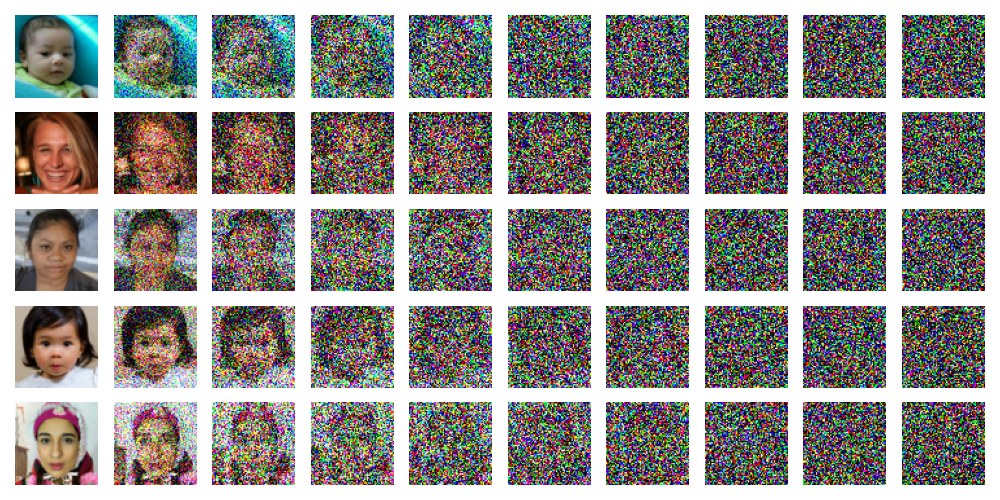
\includegraphics[width=1\textwidth]{forward2.png}
  \caption{Forward process of human64 model from $t_0$ to $t_{100}$ with linear $\beta \in(1e^{-4}, 0.05)$}
\end{figure}

Above figure shows the forward process from \(t_0\) to \(t_{100}\) with a linear \({\beta _t}\) schedule.\
The forward process is implemented in the \texttt{process.py} file, where the \texttt{q\_sample} function takes the original data and the number of steps as input and returns the noisy data at each step.\

\subsection{Scheduler}
The variance scheduler \({\beta _t}\) controls the amount of noise added at each step in the forward process.\
There are many different ways to implement this scheduler, but the most common approach is to use a linear or exponential schedule.\
The linear schedule increases the variance linearly over time, starting from a small value and gradually increasing to a larger value.\
Typically, it would look something like this: 
\[{\beta _t} = {\beta _0} + \frac{{t - 1}}{{T - 1}}({\beta _T} - {\beta _0})\]
Where \({\beta _0}\) is the initial variance, \({\beta _T}\) is the final variance, and \(T\) is the total number of steps.\
Having a larger $t$ allows for $\beta$ to be smaller (step size) while still approximating the same limiting distribution.\
Smaller time steps allow for less ambiguity in determining previous states.\
Generally, the smaller the $\beta$, the smaller the variance.\
The true reverse process will have the same functional form of the forward process using an infinitely small step size $\beta$.\

\subsection {Reverse Process}
The reverse process in diffusion models involves learning to denoise the data step by step.\
The process is similar to the forward process, but instead of adding noise, we learn to remove it.\
Mathematically, we can describe the reverse process as follows:
\[{p_\theta }({x_{0:T}}) = p({x_T})\prod\limits_{t = 1}^T {{p_\theta }({x_{t - 1}}|{x_t})} \]

Where \({p_\theta }({x_{t - 1}}|{x_t})\) is the learned transition distribution from \({x_t}\) to \({x_{t - 1}}\).\
Here, \({p(x_T)}\) is the pure noise distribution from our forward process (Gaussian) and \(\prod\limits_{t = 1}^T {{p_\theta }({x_{t - 1}}|{x_t})}\) is the product of our conditionals.\
$\theta$ represents the trainable parameters (weights, bias) of the model.\\

We can break this down further into:
\[{p_\theta }({x_{t - 1}}|{x_t}) = N({\mu _\theta }({x_t},t),\sum\limits_\theta  {({x_t},t))} \]

Which takes time $t$ and our sample $x_t$.\
The reason this is done typically is because the variance scheduler is not constant, and input $t$ allows us to account for forward process variance scheduler.\
At each time step, there are different noise levels, and the model will need to learn how to undo these steps individually.\
In short, during inference, we will start from absolute gaussian noise and begin sampling from the learned individual steps of the learned reverse process until we reach $x_0$.\

\begin{figure}[H]
  \centering
  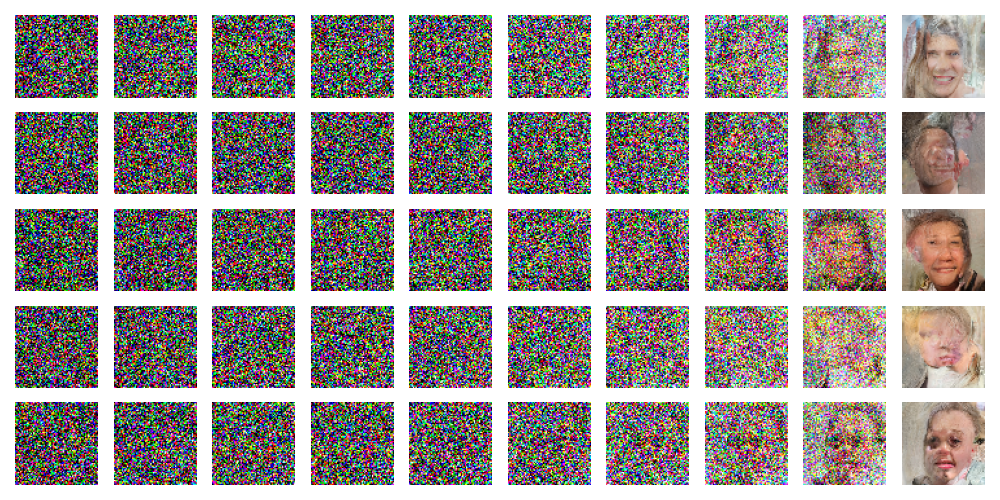
\includegraphics[width=1\textwidth]{reverse3.png}
  \caption{Reverse process of human64 model from $t_{750}$ to $t_0$ with linear $\beta \in(0.0001, 0.05)$}
\end{figure}

\subsection{Objective Function}
The objective function for training diffusion models is based on the variational lower bound on the data likelihood.\\

Let ${x_1},{x_2},...,{x_T}$ be the latent variables representing the noisy image at each step.\
Our observed value is ${x_0}$, the original image.\
With these variables, we can write the log-likelihood of the data as:
\[log(p({x_0})) >= E_{q({x_{1:T}}|{x_0})} [log(p_{\theta}({x_0}|{x_{1:T}}))] - D_{KL}(q({x_{1:T}}|{x_0})||p({x_{1:T}}))\]

Where $q({x_{1:T}}|{x_0})$ is the distribution of the noisy images given the original image, and $p({x_{1:T}})$ is the true distribution of the noisy images.\\

In other words, the first term $E_{q({x_{1:T}}|{x_0})} [log(p_{\theta}({x_0}|{x_{1:T}}))]$ is the likelihood or reconstruction term that maximizes the expected density of the data.\
It measures how well the model can reconstruct the original image ${x_0}$ given the noisy images ${x_{1:T}}$.\
A higher likelihood in this term means that the model is better at predicting the true image given the noisy observations. \\

The second term, is the Kullback–Leibler divergence: $D_{KL}(q({x_{1:T}}|{x_0})||p({x_{1:T}}))$
It is between the approximate posterior distribution \(q({x_{1:T}}|{x_0})\) and the prior distribution \(p({x_{1:T}})\).\
By minimizing this divergence, we encourage the learned distribution to be as close as possible to the true fixed prior.\
It acts like a regularizer, making sure that the model does not overfit to the training data by keeping the latent (noisy) representations close to a known one.\\

In essence, while the reconstruction term ensures the model learns to recover the image, the KL divergence term ensures that the underlying noise structure remains consistent with the assumed prior. 
This balance is crucial for the generative model to perform well both in reconstructing training images and in generating new samples from random noise.\\

We can further factor this into individual steps: 
\[{E_q}(\log {p_\theta }({x_0}|{x_{1:T}})) - {E_q}(\log \frac{{q({x_{1:T}}|{x_0})}}{{{p_\theta }({x_{1:T}})}})\]
\[{E_q}(\log {p_\theta }({x_0}|{x_{1:T}}) + \log \frac{{{p_\theta }({x_{1:T}})}}{{q({x_{1:T}}|{x_0})}})\]
\[{E_q}(\log \frac{{{p_\theta }({x_{1:T}})}}{{q({x_{1:T}}|{x_0})}})\]
\[{E_q}(\log {p_\theta }({x_T}) + \sum\limits_{t \ge 1} {\log } \frac{{{p_\theta }({x_{t - 1}}|{x_t})}}{{q({x_t}|{x_{t - 1}})}}\] 

This final form breaks the overall objective into contributions from each individual diffusion step.

\pagebreak
\section{Implementation}
After establishing the mathematical foundation for both the forward and reverse processes, a UNet-based architecture is used to learn the denoising function.\
The reverse process begins with pure Gaussian noise and iteratively removes noise until an approximation of the original image is reached.\
This iterative denoising is guided by the learned model, which is tasked with predicting the noise component at each time step.

\subsection{Dataset and Pre-processing}
The two datasets that were used to train the model are the Cat vs Dog \cite{dog} and Flickr-Faces-HQ \cite{faces} datasets from Kaggle.\
The first dataset contains 500 512x512 pixel images for both cats and dogs .\
For the purpose of this model, I decided to only use the 500 dog images.\
Since I am memory constrained, the images were downsampled to both 32x32 and 64x64 pixel images for training.\
The second dataset contains around 52k 512x512 pixel images of a variety of human faces.\
Since human faces are a bit more sophisticated, I decided to try and downsample the images to 64x64 pixels, and utilize 10k images for training.\
The images are then converted to numpy arrays, with 3 different channels for red, green, and blue and converted into tensors.\
Finally, using these tensors, the transformations and normalization between the range of [0, 1] are applied on the GPU.\

\begin{figure}[H]
  \centering
  \begin{subfigure}{0.5\textwidth}
    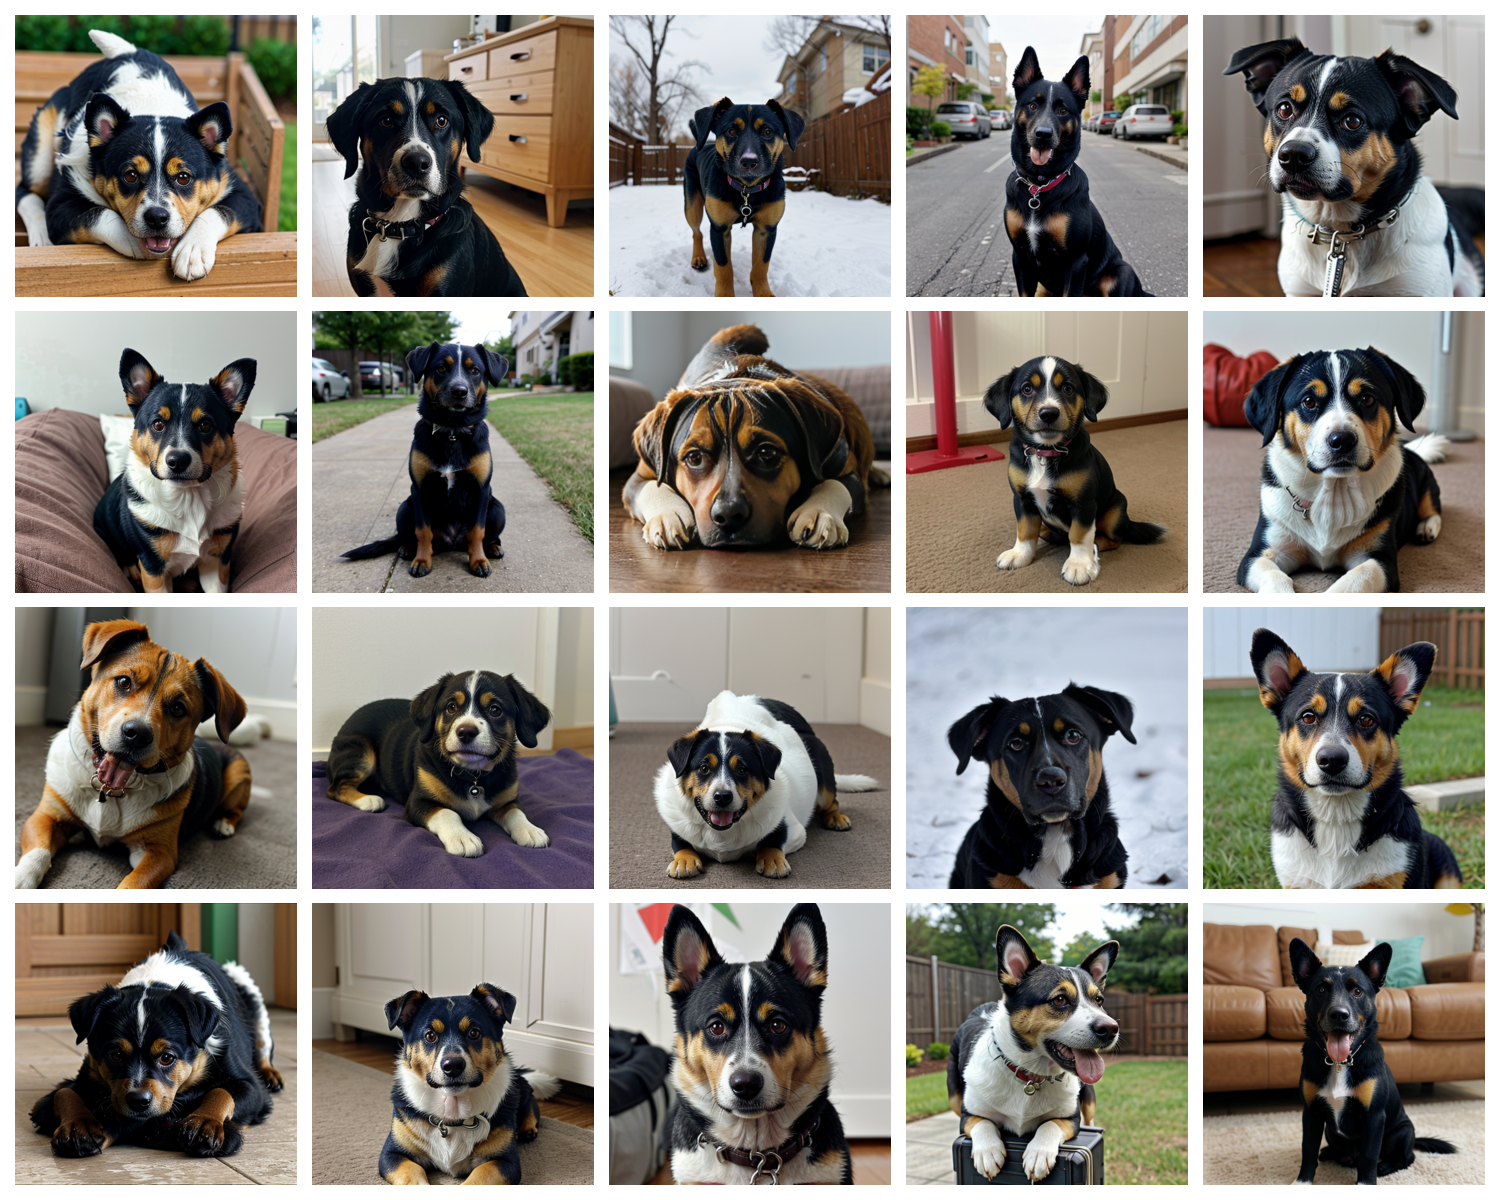
\includegraphics[width=1\textwidth]{dogs.png}
  \end{subfigure}%
  \begin{subfigure}{0.5\textwidth}
    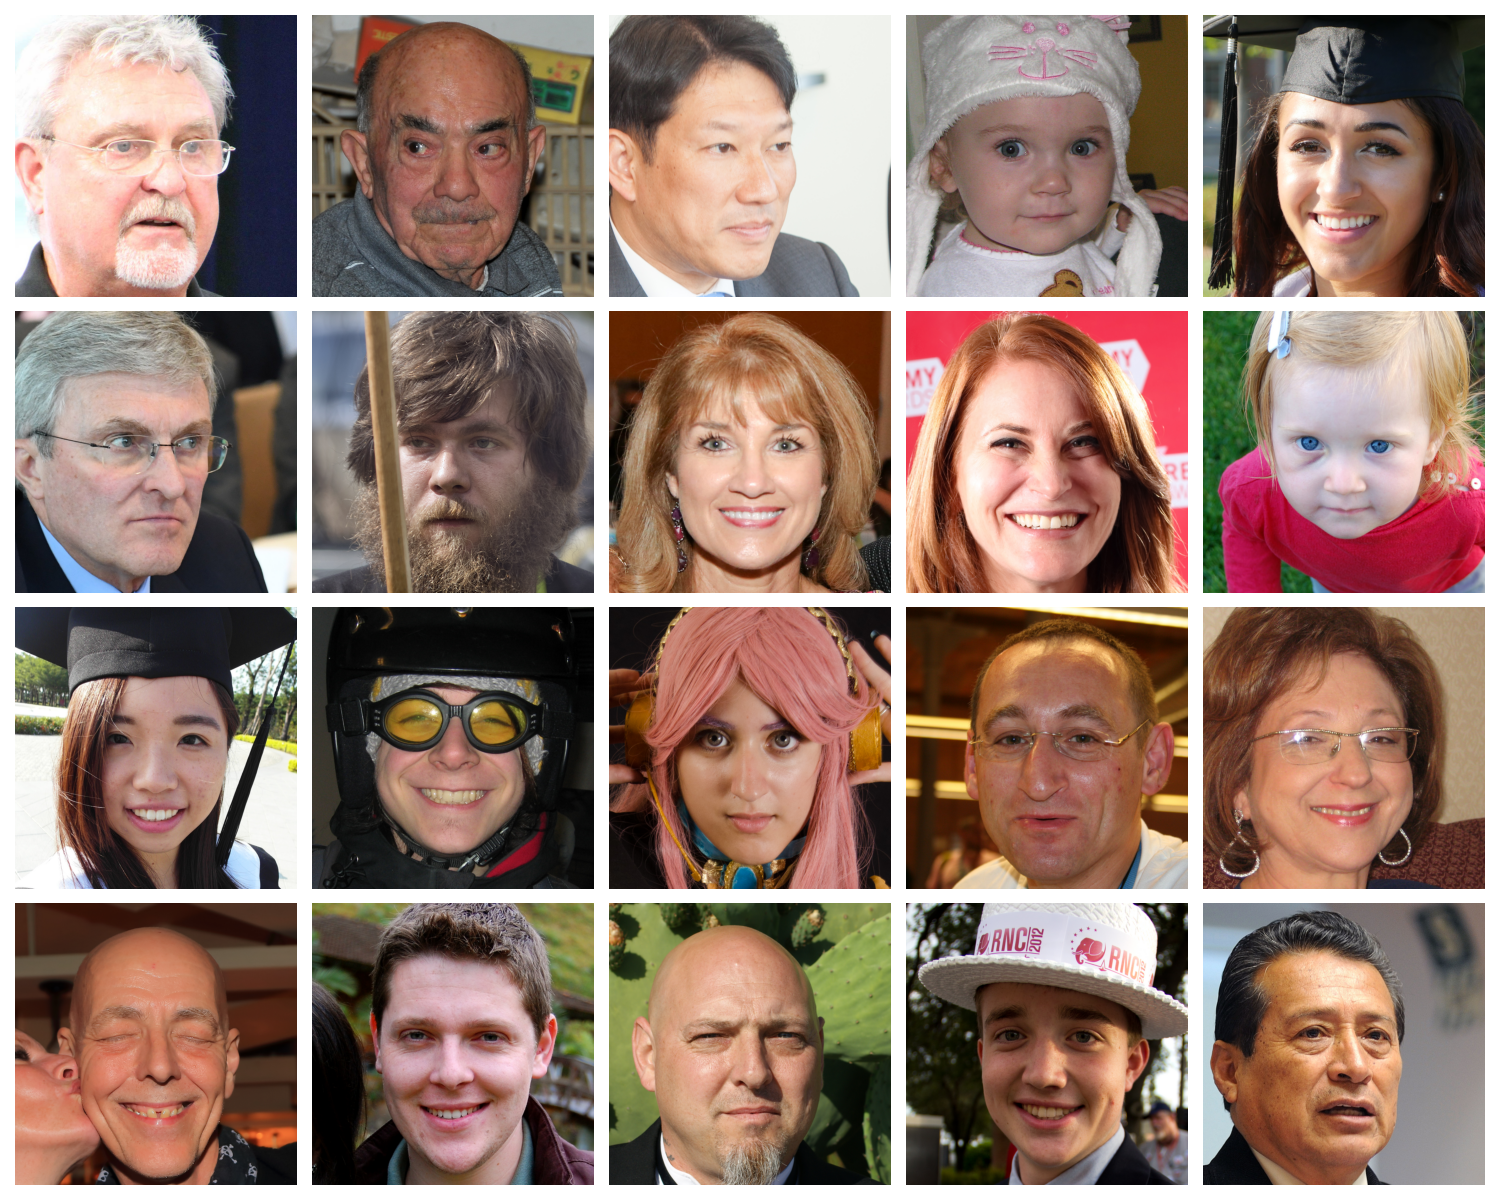
\includegraphics[width=1\textwidth]{face.png}
  \end{subfigure}%
  \caption{Sample images from training datasets: Left: Dog vs Cat Dataset \cite{dog} Right: Flickr-Faces-HQ Dataset \cite{faces}}
\end{figure}

\subsection{UNet Architecture}
To predict the noise effectively, I used the same UNet architecture found in the DDPM paper \cite{ho}.\
This architecture was originally created for biomedical image segmentation \cite{unet}.\
At a high level, it is a convolutional network that consists of two parts: 
The first part is the encoder, which progressively downsamples the input image to capture high-level features.\
Then, there is the decoder which projects the lower resolution features learned by the encoder onto the higher level pixel space to reconstruct the image.\
For the purpose of this model, the implementation follows closely to the original UNet architecture with a few adjustments.\\

The rest of the model consists of four major parts:\\

\textbf{Time Embedding:} Firstly, there is a time embedding function that encodes the time step information into a fixed-size vector.\
I used a sinusoidal function to encode the time step, which is then passed through a linear layer to obtain the final embedding.\
This embedding is then concatenated with the feature maps at each time step in the decoder.\
This part is important since the denoising function is dependent on the time step.\
By embedding the time step, the model can learn to condition its predictions based on the current noise level at the specific time step.\\

\textbf{Downsampling:} This second module is the downsampling layer which is your standard convolutional layer that reduces the spatial resolution of the input image.\
This is then followed by a leaky ReLU activation function and a batch normalization layer.\\

\textbf{Upsampling:} This increases the spatial resolution of the feature maps back to the original size, for reconstructing the detailed structure of the image. \
During upsampling, the network also uses skip connections (Residual Block) to combine fine-grained information from the corresponding downsampling layers. \\

\textbf{Residual Block:} The residual block is for the residual mapping between the input and output of the block.\
Because at each upsample and downsample step, the input and output will be at the same resolution, the residual block "reminds" the network of what it is trying to learn initially.\
As for any convolutional step, you will lose information every time you downsample and by adding this block, it mitigates the loss of information from layer to layer.\
This is similar to the ResNet architecture \cite{resnet} which uses skip connections to allow gradients to flow more easily through the network during training.\\

The model is implemented in the \texttt{model.py} file, where the \texttt{UNet} class defines the architecture and the forward pass.\
First, the input tensor is passed into the embedding function.\
It then gets passed through two downsampling layers, with each layer having double the amount of base channels.\
After that, the tensor is passed through the two upsample layers, which combines the feature maps from the downsampling layers using skip connections.\
Finally, the output is passed through a final convolutional layer to produce the denoised image.\

\subsection{Forward Process}

The implementation of the forward process is quite simple.\
Using the forward process equation that was derived in section 2.1.\
First, the linear beta schedule is defined depending on the number of time steps and the cumulative product of the alphas are pre-computed.\
Since we are using a fixed scheduled $\beta_t$, we can sample the forward process in closed form without needing to go through the entire chain using the equation from Section 2.1.\
This allows us to compute the noisy images at any arbitrary time step without iterating through all previous steps.\
Since this task is embarrassingly parallel, tensors are allocated on the GPU and operations are vectorized to leverage parallel computation.\

\subsection{Reverse Process}

In the reverse process, we precompute quantities such as the posterior variance for each timestep.\
This variance is used to add an appropriate amount of stochastically during each reverse step.\
By precomputing these values based on the same noise schedule as the forward process, it makes sure that the scheduler is consistent with the forward process.\
The reverse process uses the noise prediction model to compute the mean of the reverse transition: 

\[{\mu _\theta }({x_t},t) = \frac{1}{{\sqrt {{\alpha _t}} }}({x_t} - \frac{{1 - {\alpha _t}}}{{\sqrt {1 - \overline {{\alpha _t}} } }}{\epsilon _\theta }({x_t},t))\]

Where ${\epsilon _\theta }({x_t},t)$ is the predicted noise from the model at time $t$. \\

For timesteps $t > 0$, noise is added based on the posterior variance to maintain the stochastic nature of the diffusion process.\
This design choice reflects the inherent uncertainty in the reverse process and prevents the reverse transitions from becoming overly deterministic, which is important for generalization (More random samples).

\subsection{Limitations and Modfications}
Due to GPU memory constraints, I opted for a reduced number of base channels and time embedding steps in the convolutional layers, output resolution, batch sizes, and timesteps.\
By choosing a lower base channel count (e.g., 256-512 instead of 1024+), I significantly decreased the number of parameters, making it feasible to train the network on a limited VRAM without compromising (much) on the overall structure of the model for lower resolutions.\\
I also lowered the dimensionality of the time embedding to 512 dimensions.\
This reduction helped in minimizing the computational overhead associated with processing temporal information, while still providing sufficient detail to effectively incorporate the diffusion timestep into the denoising process.\\

Training instability was a further challenge that I addressed through careful tuning of both the learning rate, number of timesteps, and batch sizes.\
Finding the right parameters for both of these is hard since I had to do a lot of trial and error to find what works best.\
For each trial, I would have to train the model for a few hours to even see if it was working.\
The batch sizes were especially important since too little would cause the model to train slower and potentially overfit, and too much wreak havoc on my graphics card.\
By setting the learning rate to \(1e^{-4}\), I ensured that the model’s parameter updates remained small and controlled, thereby promoting a more stable convergence and preventing oscillations or divergence during training.\
For most of the models, I stuck to between 750 and 1000 time steps to balance the trade-off between training time and the quality of generated samples.

\pagebreak
\section{Outcomes}

The following figures show the results of the trained model on the dog and human faces datasets.\
The first dog32 model was trained on 32x32 images with $t=1000$ steps and a linear beta schedule of $\beta \in(1e^{-4}, 0.02)$.\

\begin{figure}[H]
  \centering
  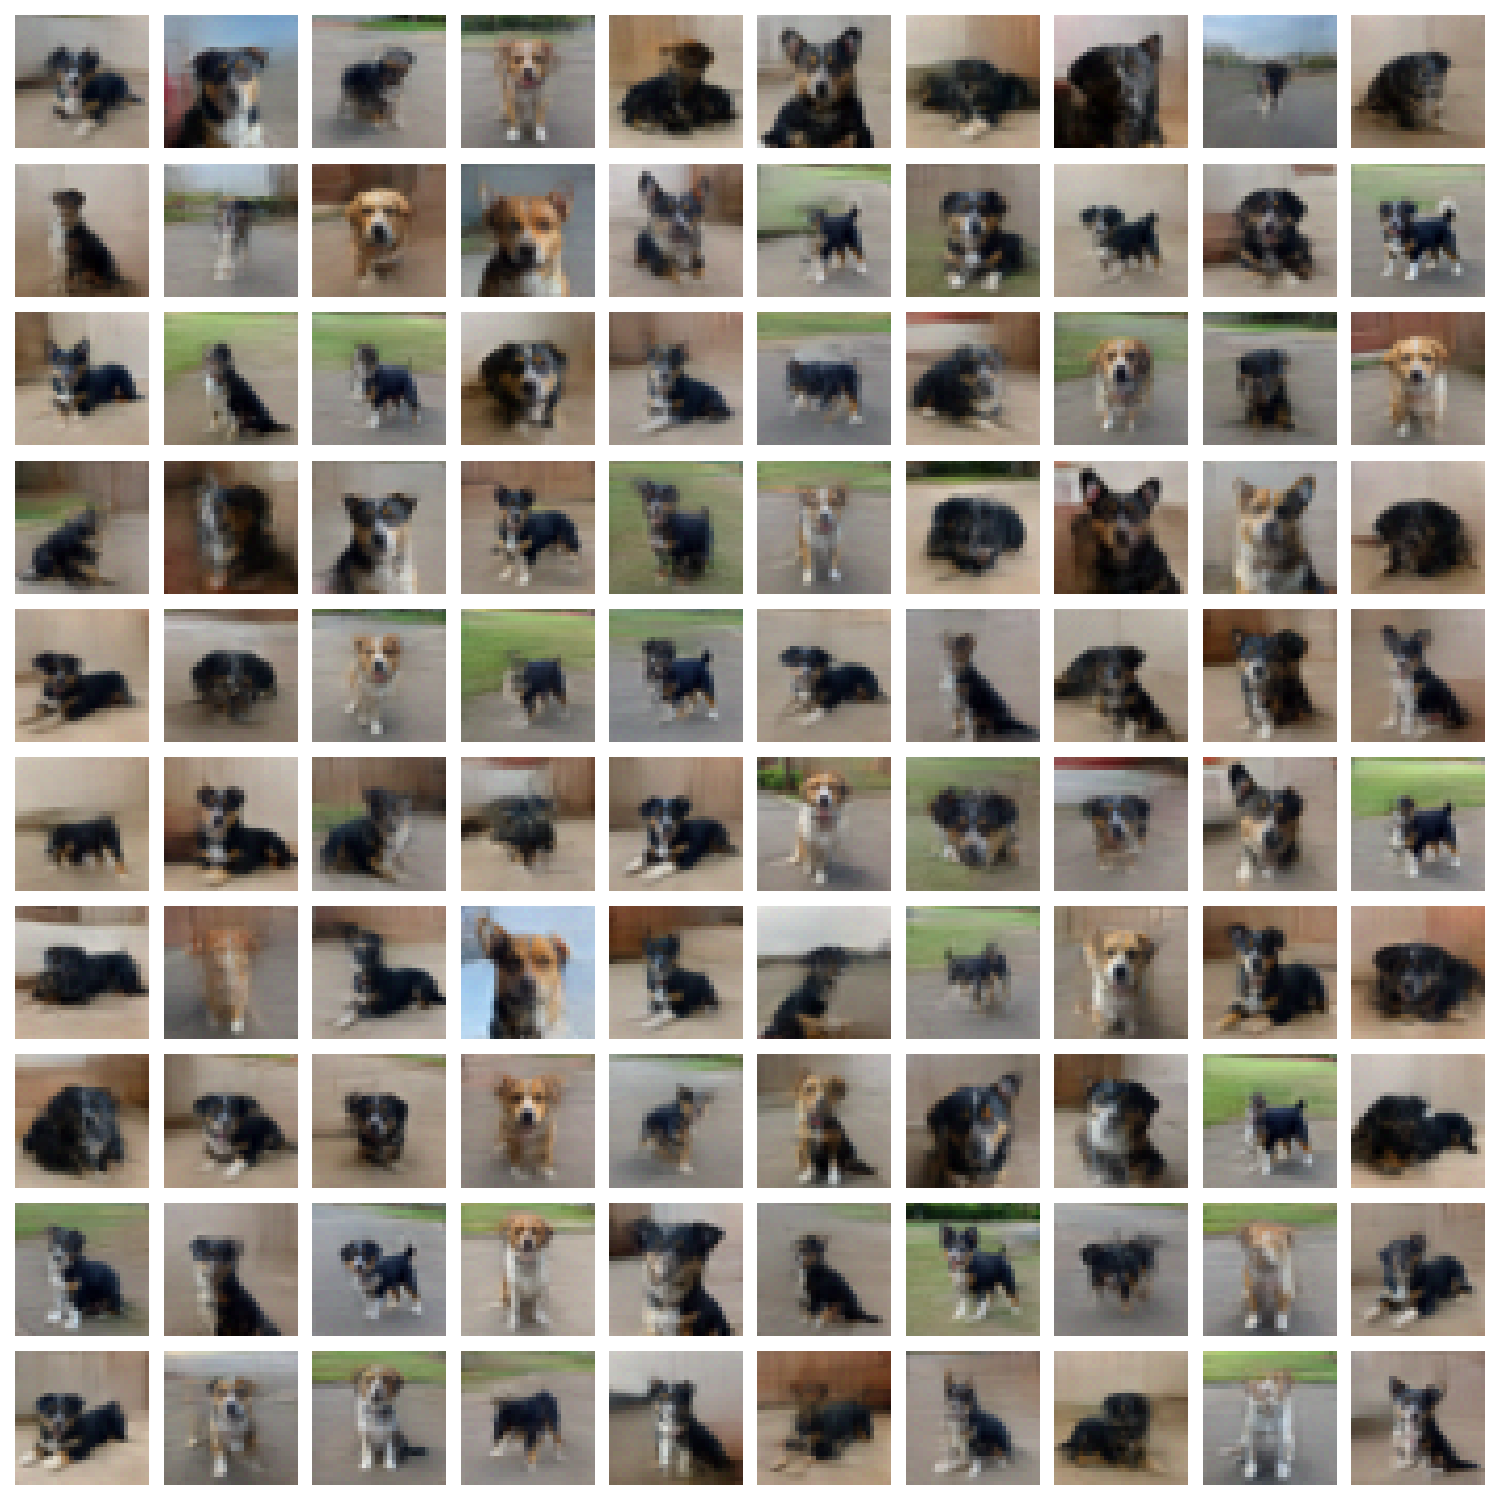
\includegraphics[width=1\textwidth]{dog32.png}
  \caption{Trained dog32 model, $t=1000$, in\_channels = $256$, batch\_size = 64, lr$=1e^{-4}$, linear $\beta \in(1e^{-4}, 0.02)$}
\end{figure}

Due to the small image size, the model was able to learn the denoising function quite well.\
The generated samples were quite similar to the training dataset however, since it was only trained on 500 different samples, the generated images were very similar.\
This smaller model was used to test the implementation and ensure that the model was able to learn the denoising function.\
Finding a balance for the base channels and the number of residual blocks was difficult since it is different for each dataset.\
Setting the base channels too high or increasing the number of residual blocks would result in higher computational costs, longer train times, and could lead to overfitting.\
Setting it too low would result in the model not being able to learn the denoising function effectively.\\

The following images below shows the progression of the "human64" model.\
It was trained on 64x64 images with $t=750$ steps and a linear beta schedule of $\beta \in(1e^{-4}, 0.01)$.\
Instead of only 500 samples, this model was trained on 10k samples, which allowed for a much larger variety of images.\
Additionally, I upped the resolution to 64x64, however due to GPU memory constraints, I had to reduce the batch size significantly to 16.\
Initially, at the start of training, it caused the model to generate black images, however after upping the base channels on the model by $50\%$, it was able to learn the denoising functions a little better.\

\begin{figure}[H]
  \centering
  \begin{subfigure}{0.5\textwidth}
    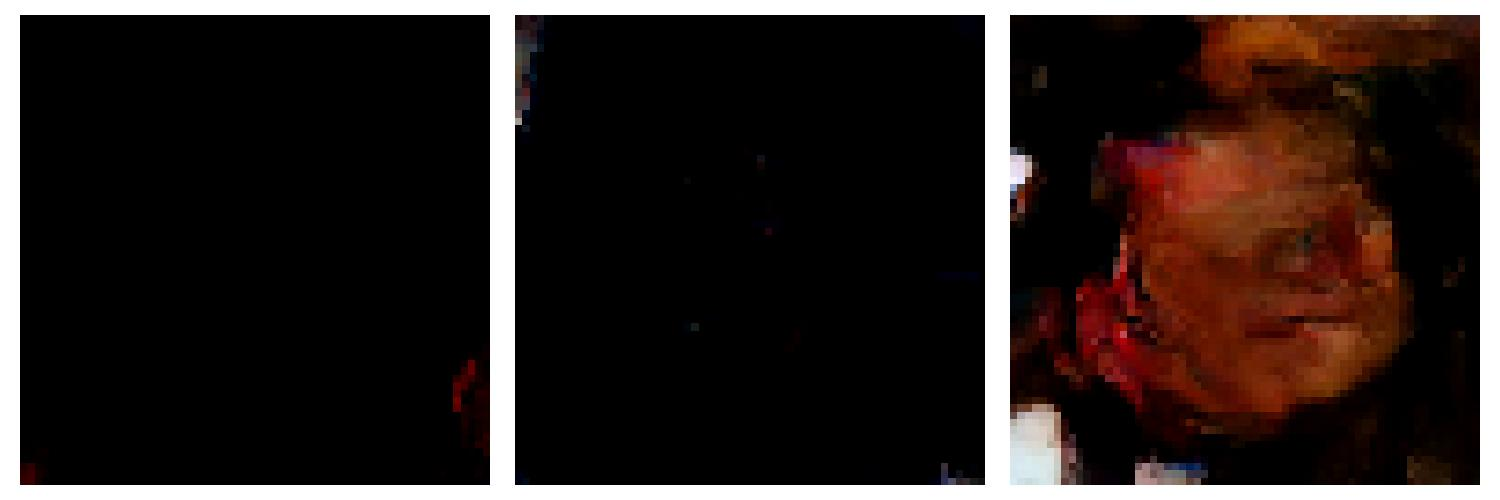
\includegraphics[width=1\textwidth]{human5k.jpg}
  \end{subfigure}%
  \begin{subfigure}{0.5\textwidth}
    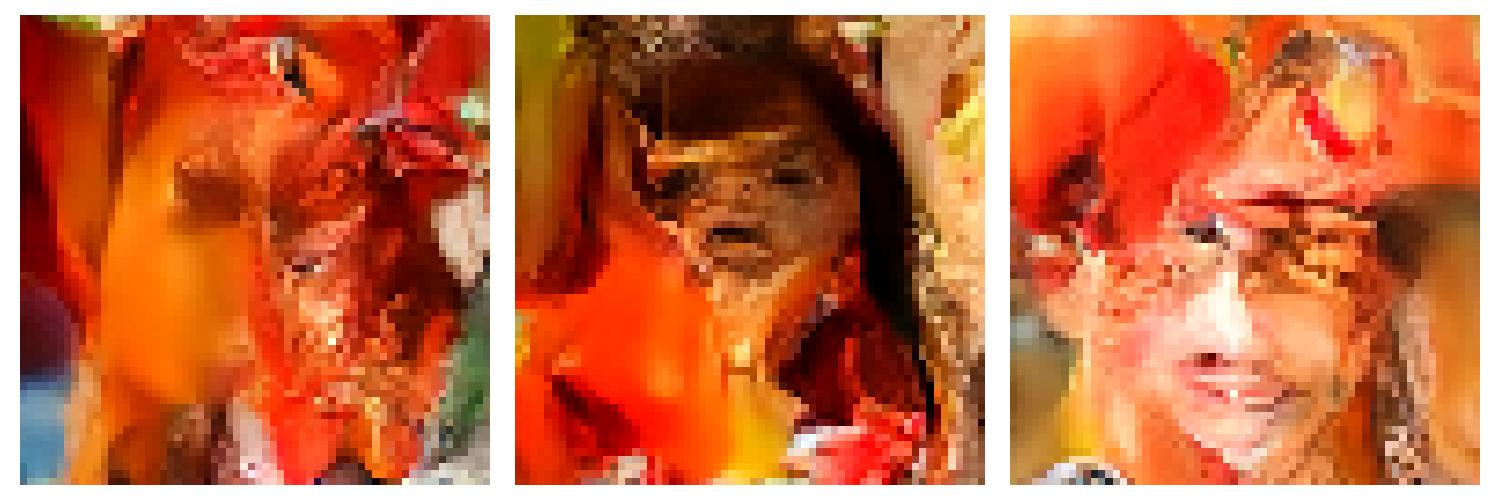
\includegraphics[width=1\textwidth]{human10k.jpg}
  \end{subfigure}
  \begin{subfigure}{0.5\textwidth}
    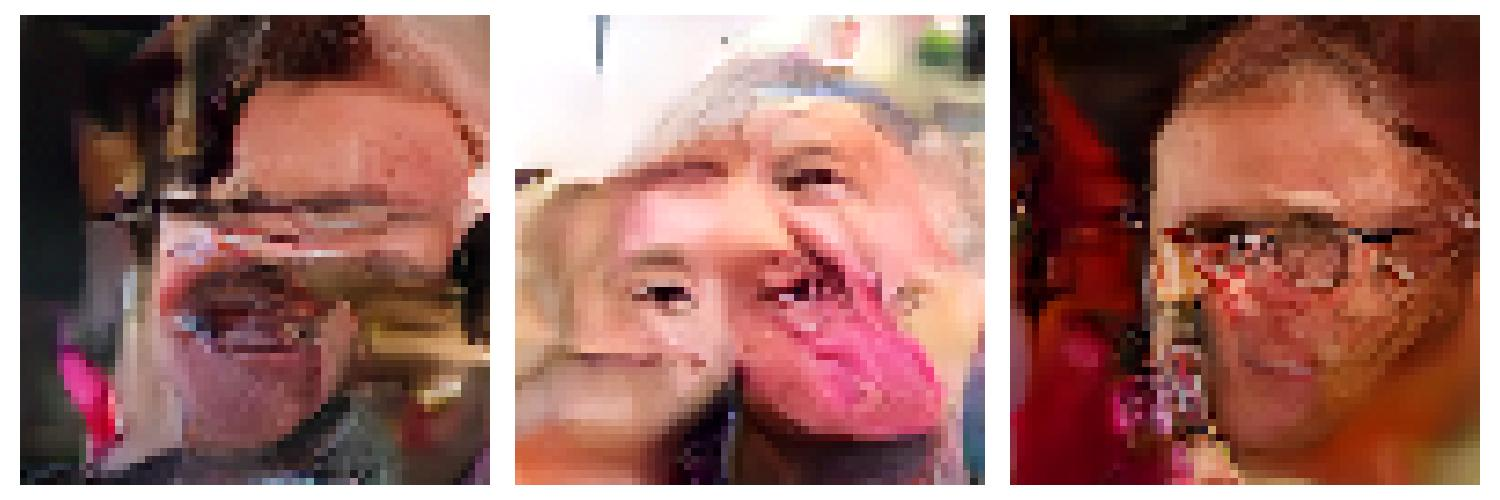
\includegraphics[width=1\textwidth]{human20k.jpg}
  \end{subfigure}%
  \begin{subfigure}{0.5\textwidth}
    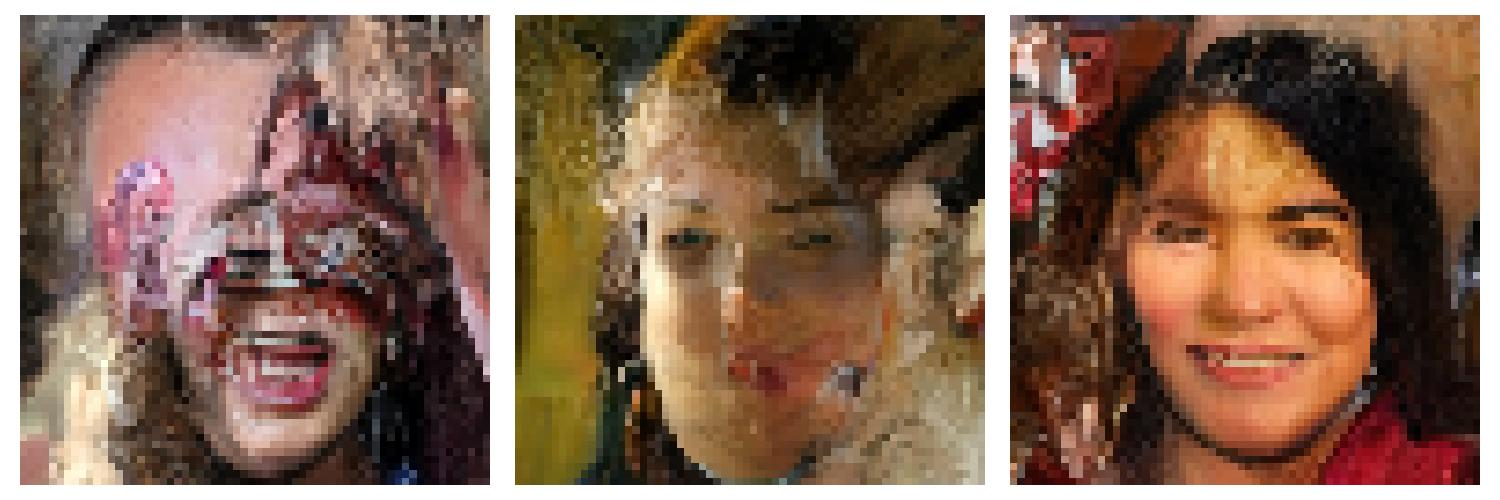
\includegraphics[width=1\textwidth]{human90k.jpg}
  \end{subfigure}
  \caption{Progression of human64 model from 5k to 90k epochs. $t=750$, base\_channels = $384$, batch\_size = 16, lr$=1e^{-4}$, linear $\beta \in(1e^{-4}, 0.02)$}
\end{figure}

\begin{figure}[H]
  \centering
  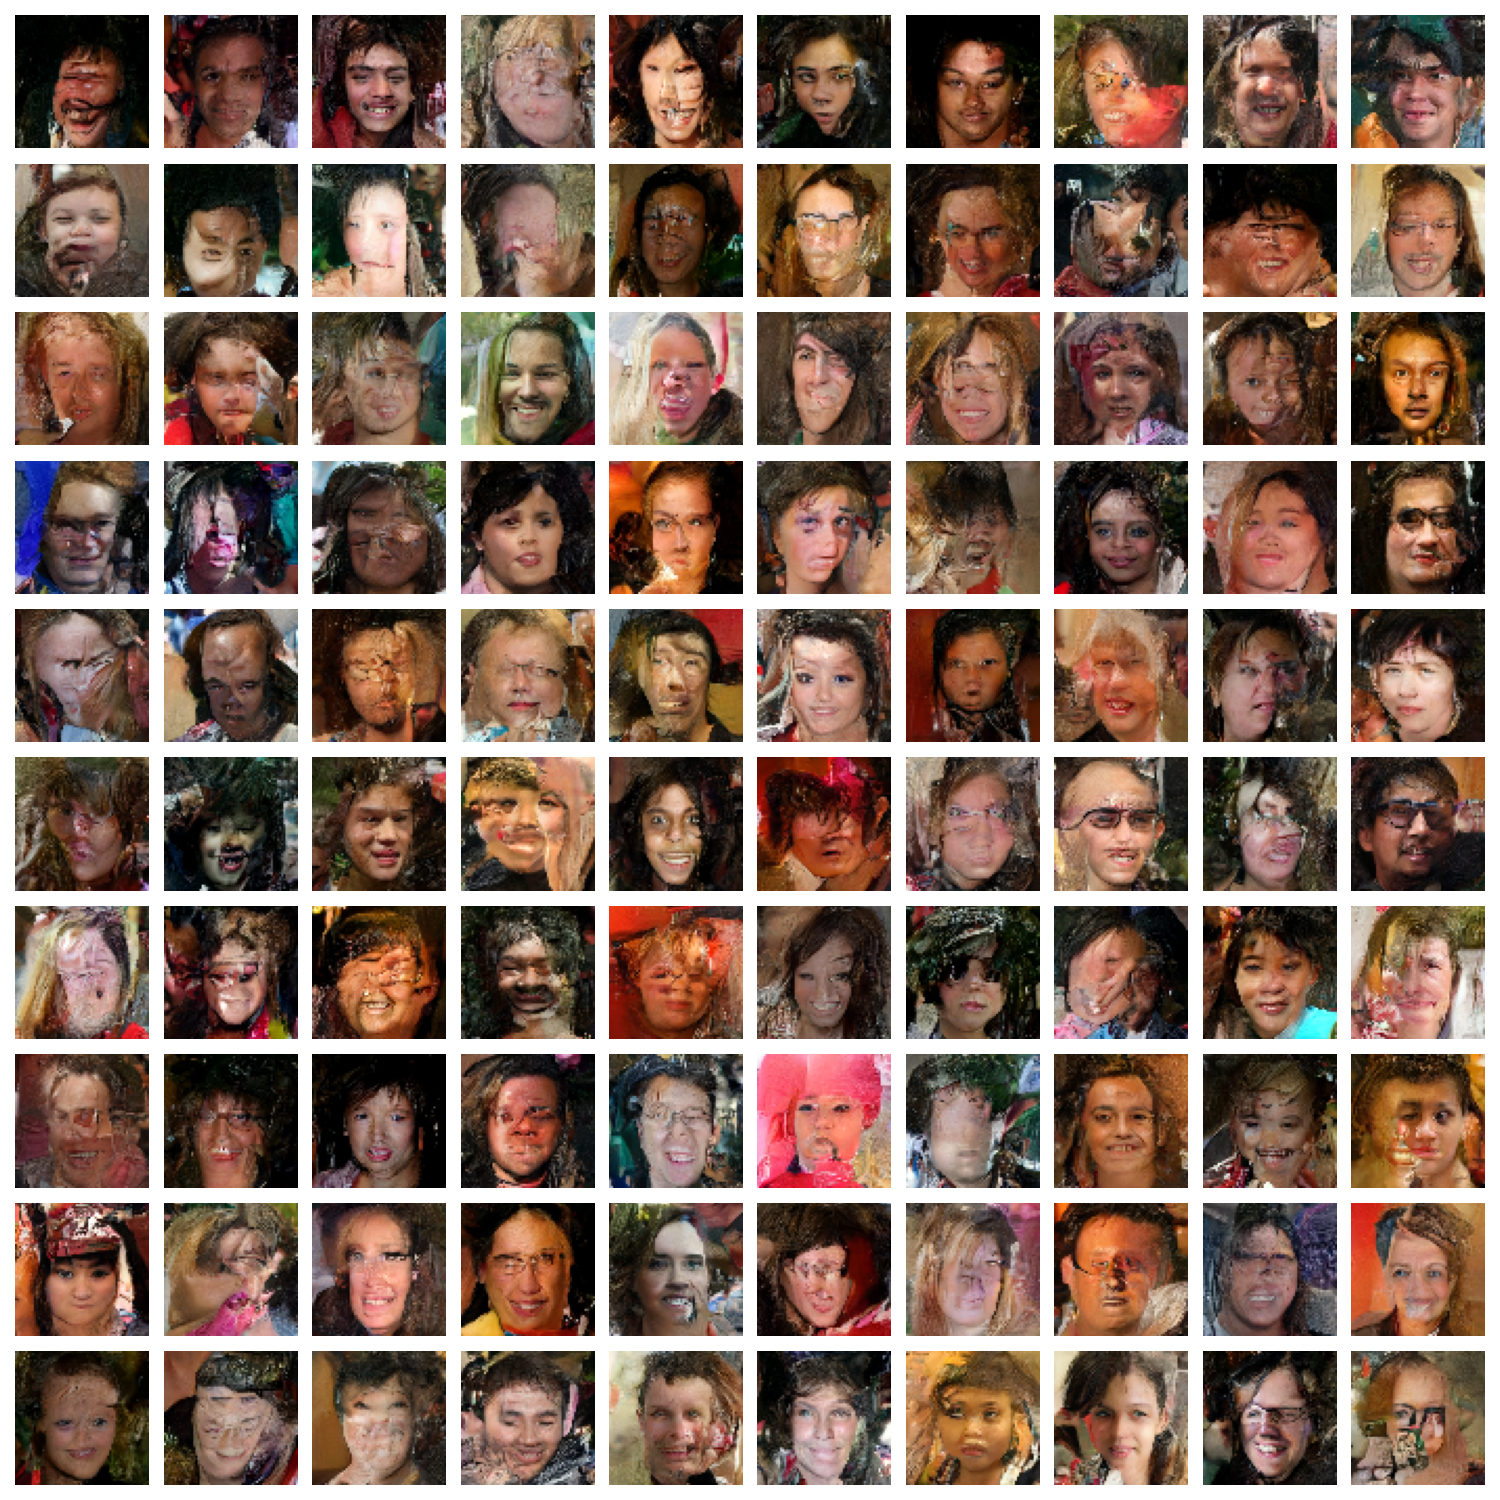
\includegraphics[width=1\textwidth]{human64.png}
  \caption{Trained human64 model, $t=750$, base\_channels = $384$, batch\_size = 16, lr$=1e^{-4}$, linear $\beta \in(1e^{-4}, 0.02)$}
\end{figure}

Although the result is not perfect, it is able to generate a variety of human faces with different features and backgrounds.\
If I was not limited by time and VRAM, the model could be trained for longer, on higher base channels, with the full 50k samples on higher batch sizes.\
Additionally, I initially tried to use more residual blocks since the resolution is higher, however it caused the model to generate random noise (perhaps overfitting), while also taking up significantly more VRAM.\
Given the constraints of the project, I am satisfied with the results.\
The model was able to learn the denoising function and generate samples that are visually similar to the training data.\\

\vspace{15.5cm}
Note: This program is written with CUDA in mind so a Nvidia GPU is required.\
Alterations could be made apple MPS and possibly ROCm (Not sure I don't have Radeon GPU). Don't run on CPU unless you want to wait forever.

\pagebreak
\begin{thebibliography}{0}

  \bibitem{dog}
  AnthonyTherrien,  yavuzibr. (2024, September 28). Dog vs cat. Kaggle. \url{https://www.kaggle.com/datasets/anthonytherrien/dog-vs-cat}

  \bibitem{resnet}
  He, K., Zhang, X., Ren, S., \& Sun, J. (2015, December 10). Deep residual learning for image recognition. arXiv.org. https://arxiv.org/abs/1512.03385 

  \bibitem{ho}
  Ho, J., Jain, A., \& Abbeel, P. (2020, December 16). Denoising Diffusion Probabilistic models. arXiv.org. \url{https://doi.org/10.48550/arXiv.2006.11239} 

  \bibitem{nichol}
  Nichol, A., \& Dhariwal, P. (2021, February 18). Improved denoising diffusion probabilistic models. arXiv.org. \url{https://arxiv.org/abs/2102.09672}

  \bibitem{unet}
  Ronneberger, O., Fischer, P., \& Brox, T. (2015, May 18). U-Net: Convolutional Networks for Biomedical Image Segmentation. arXiv.org. \url{https://arxiv.org/abs/1505.04597}

  \bibitem{faces}
  Rougetet, A. (2020, March 9). Flickr-Faces-HQ Dataset (FFHQ). Kaggle. \url{https://www.kaggle.com/datasets/arnaud58/flickrfaceshq-dataset-ffhq}

\end{thebibliography}

\pagebreak
\subsection*{Appendix}
The following are some more figures generated by the models trained:\

\begin{figure}[H]
  \centering
  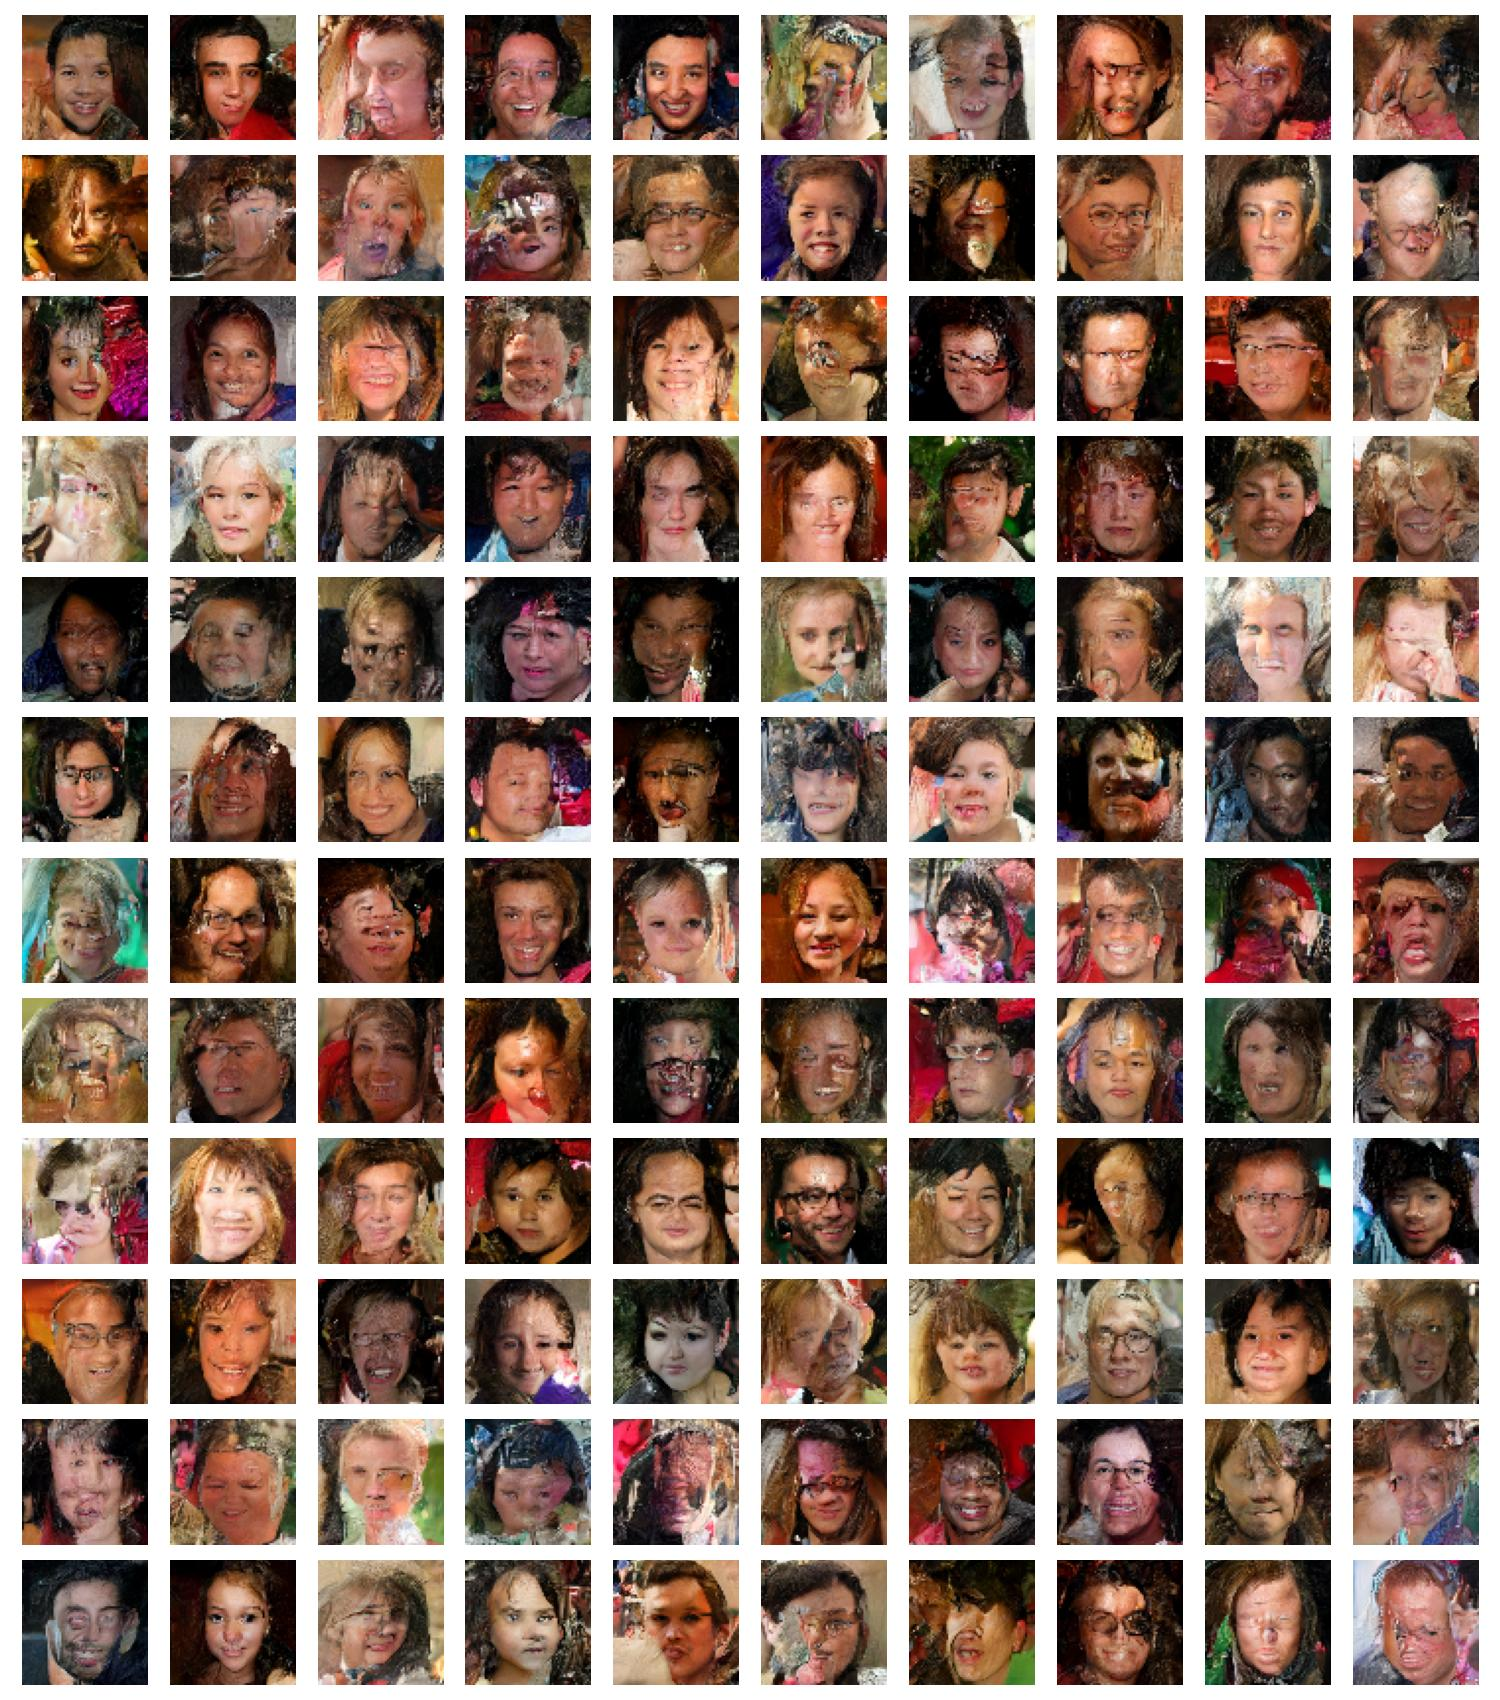
\includegraphics[width=1\textwidth]{human64ext.jpg}
  \caption{human64 model, $t=750$, base\_channels = $384$, time\_emb\_dim = $512$, batch\_size = 16, lr$=1e^{-4}$, linear $\beta \in(1e^{-4}, 0.02)$}
\end{figure}


\begin{figure}[H]
  \centering
  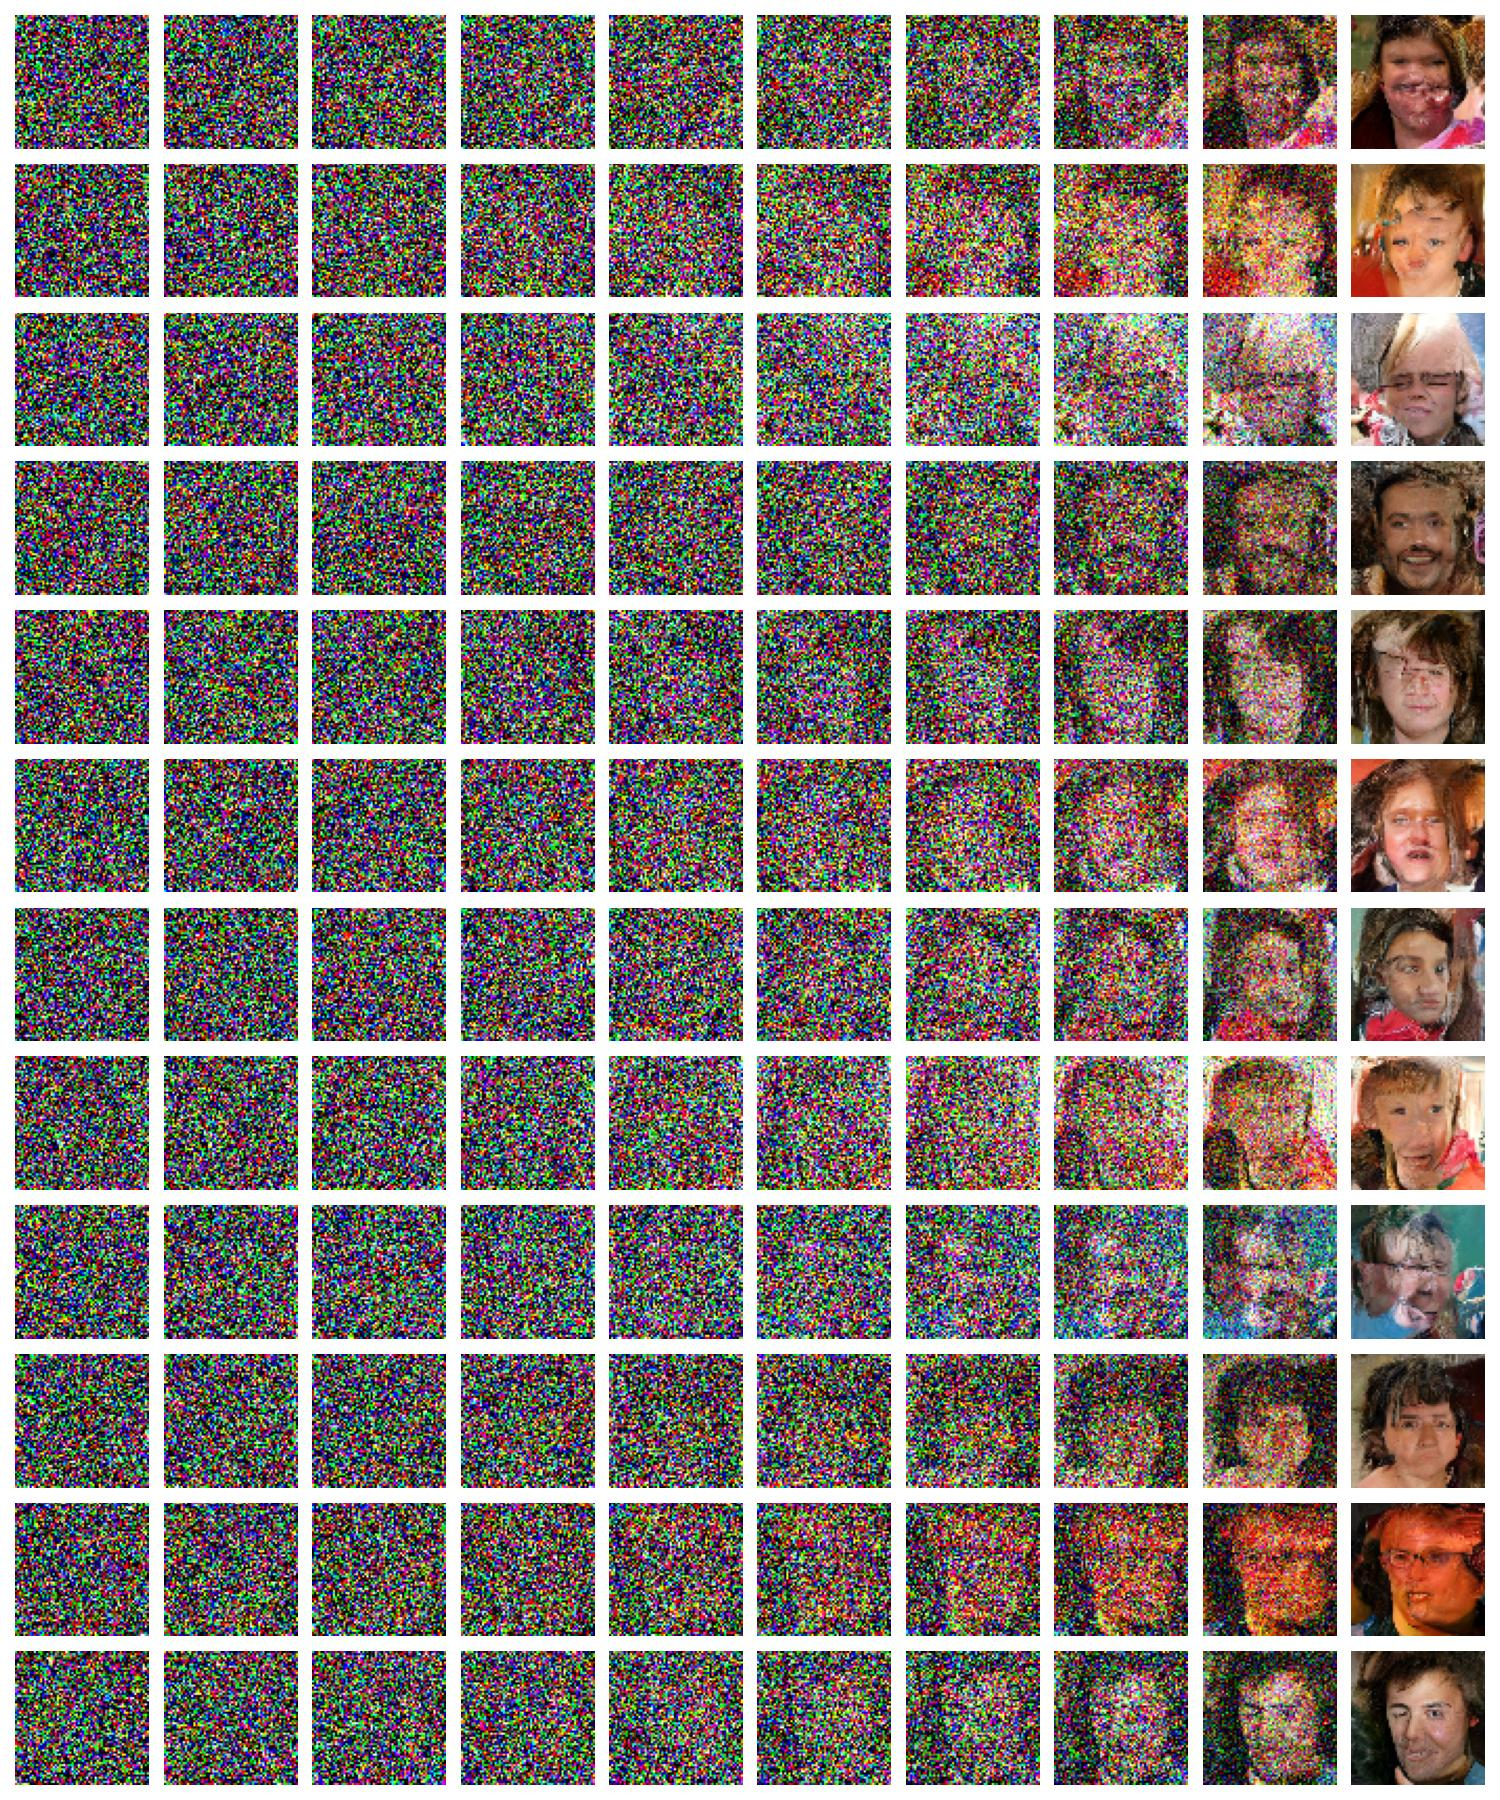
\includegraphics[width=1\textwidth]{human64rev.jpg}
  \caption{human64 model reverse process, 75 step transitions, $t=750$, base\_channels = $512$, time\_emb\_dim = $512$, batch\_size = 16, lr$=1e^{-4}$, linear $\beta \in(1e^{-4}, 0.02)$}
\end{figure}

\begin{figure}[H]
  \centering
  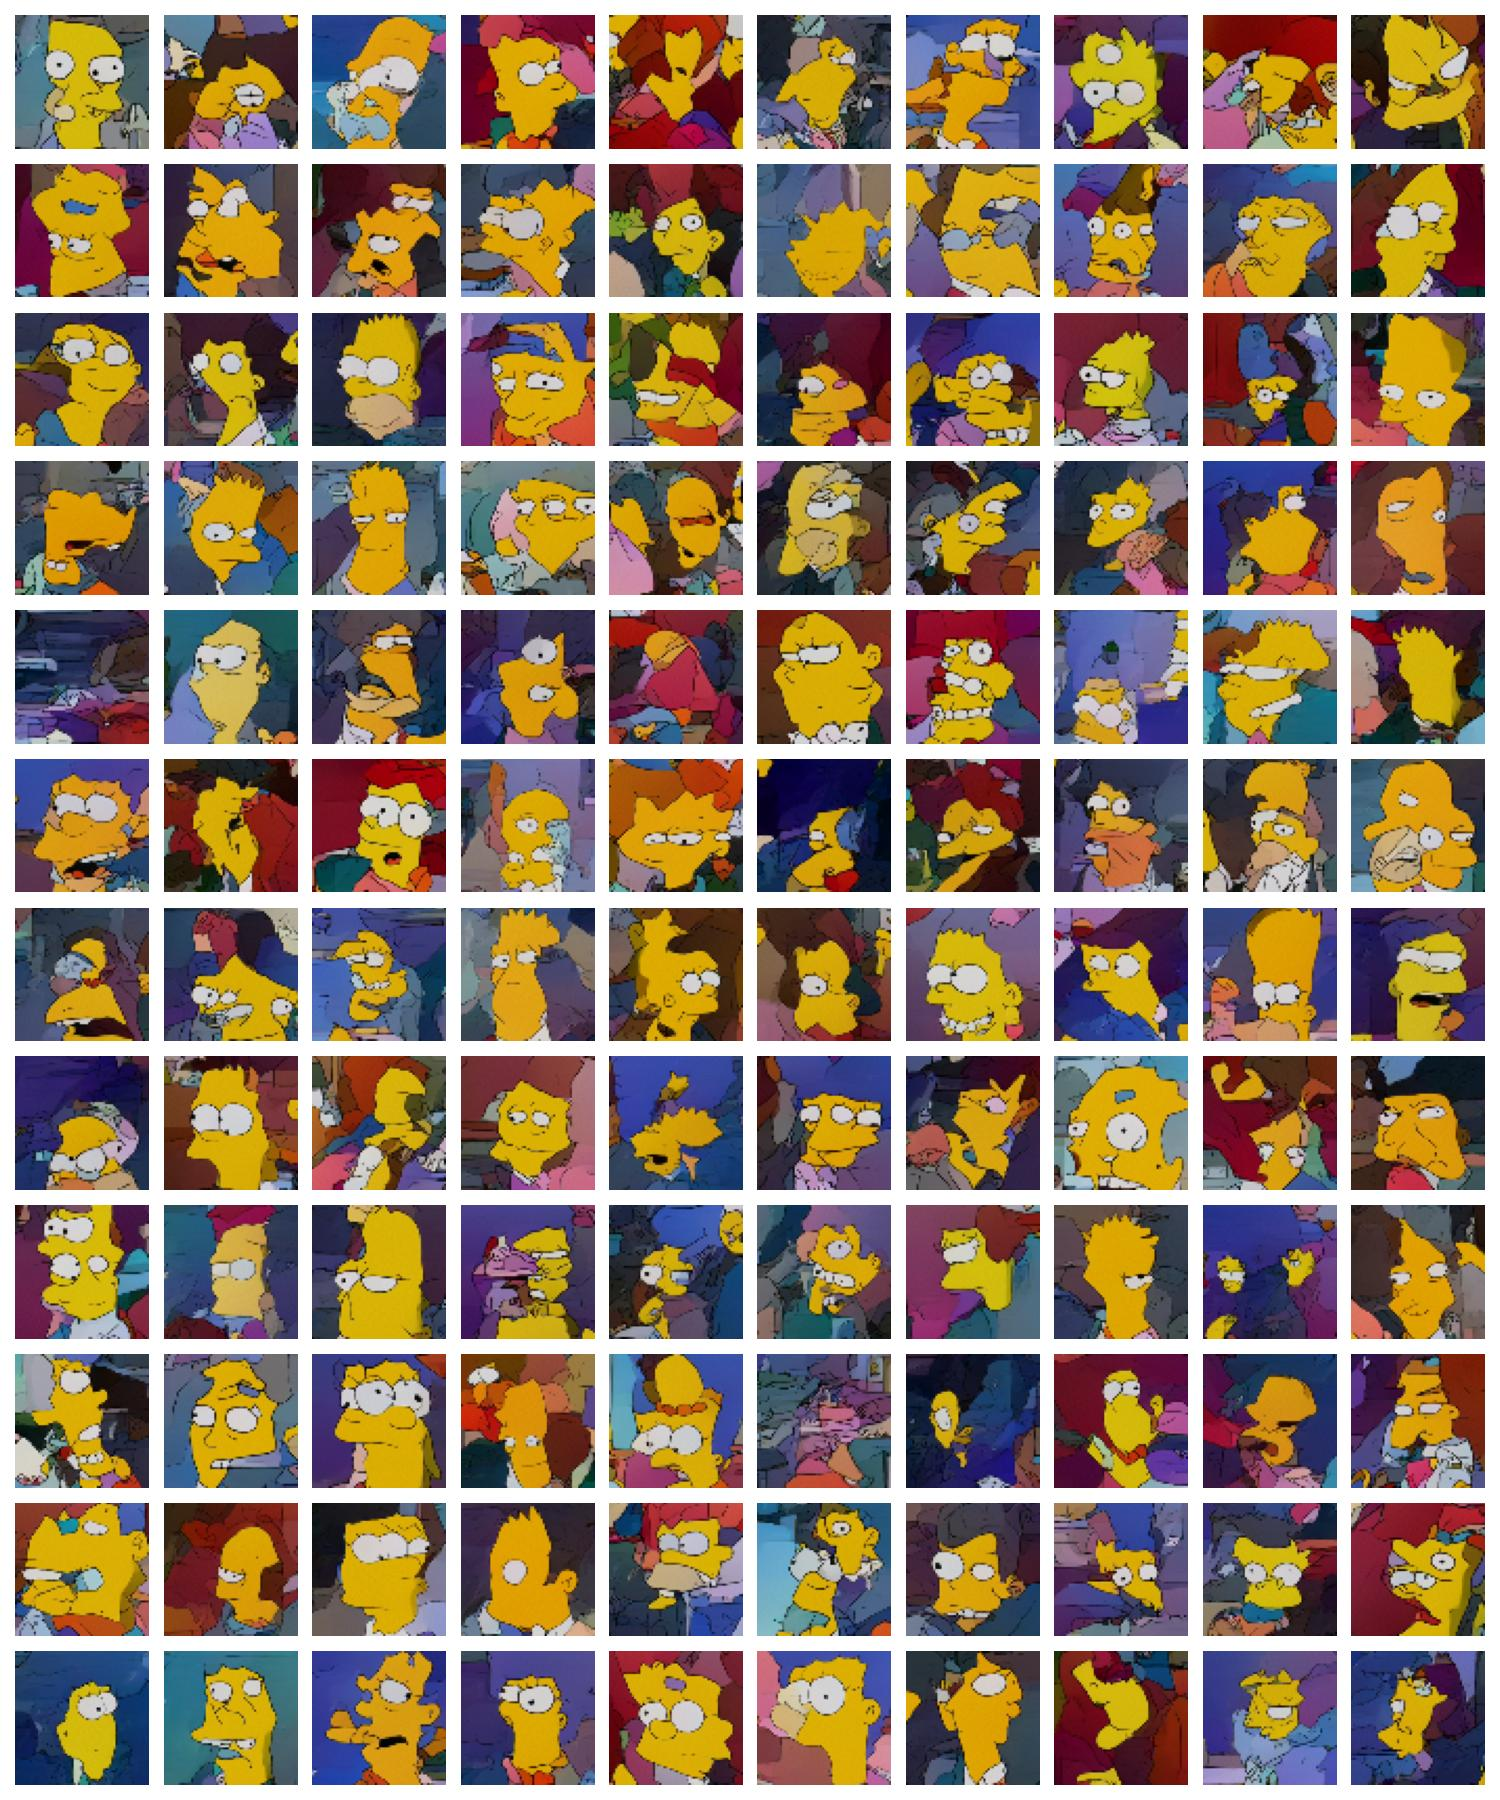
\includegraphics[width=1\textwidth]{simp64ext.jpg}
  \caption{drunkSimpson64 model, $t=500$, base\_channels = $512$, time\_emb\_dim = $512$, batch\_size = 16, lr$=1e^{-4}$, linear $\beta \in(1e^{-4}, 0.02)$}
\end{figure}

\begin{figure}[H]
  \centering
  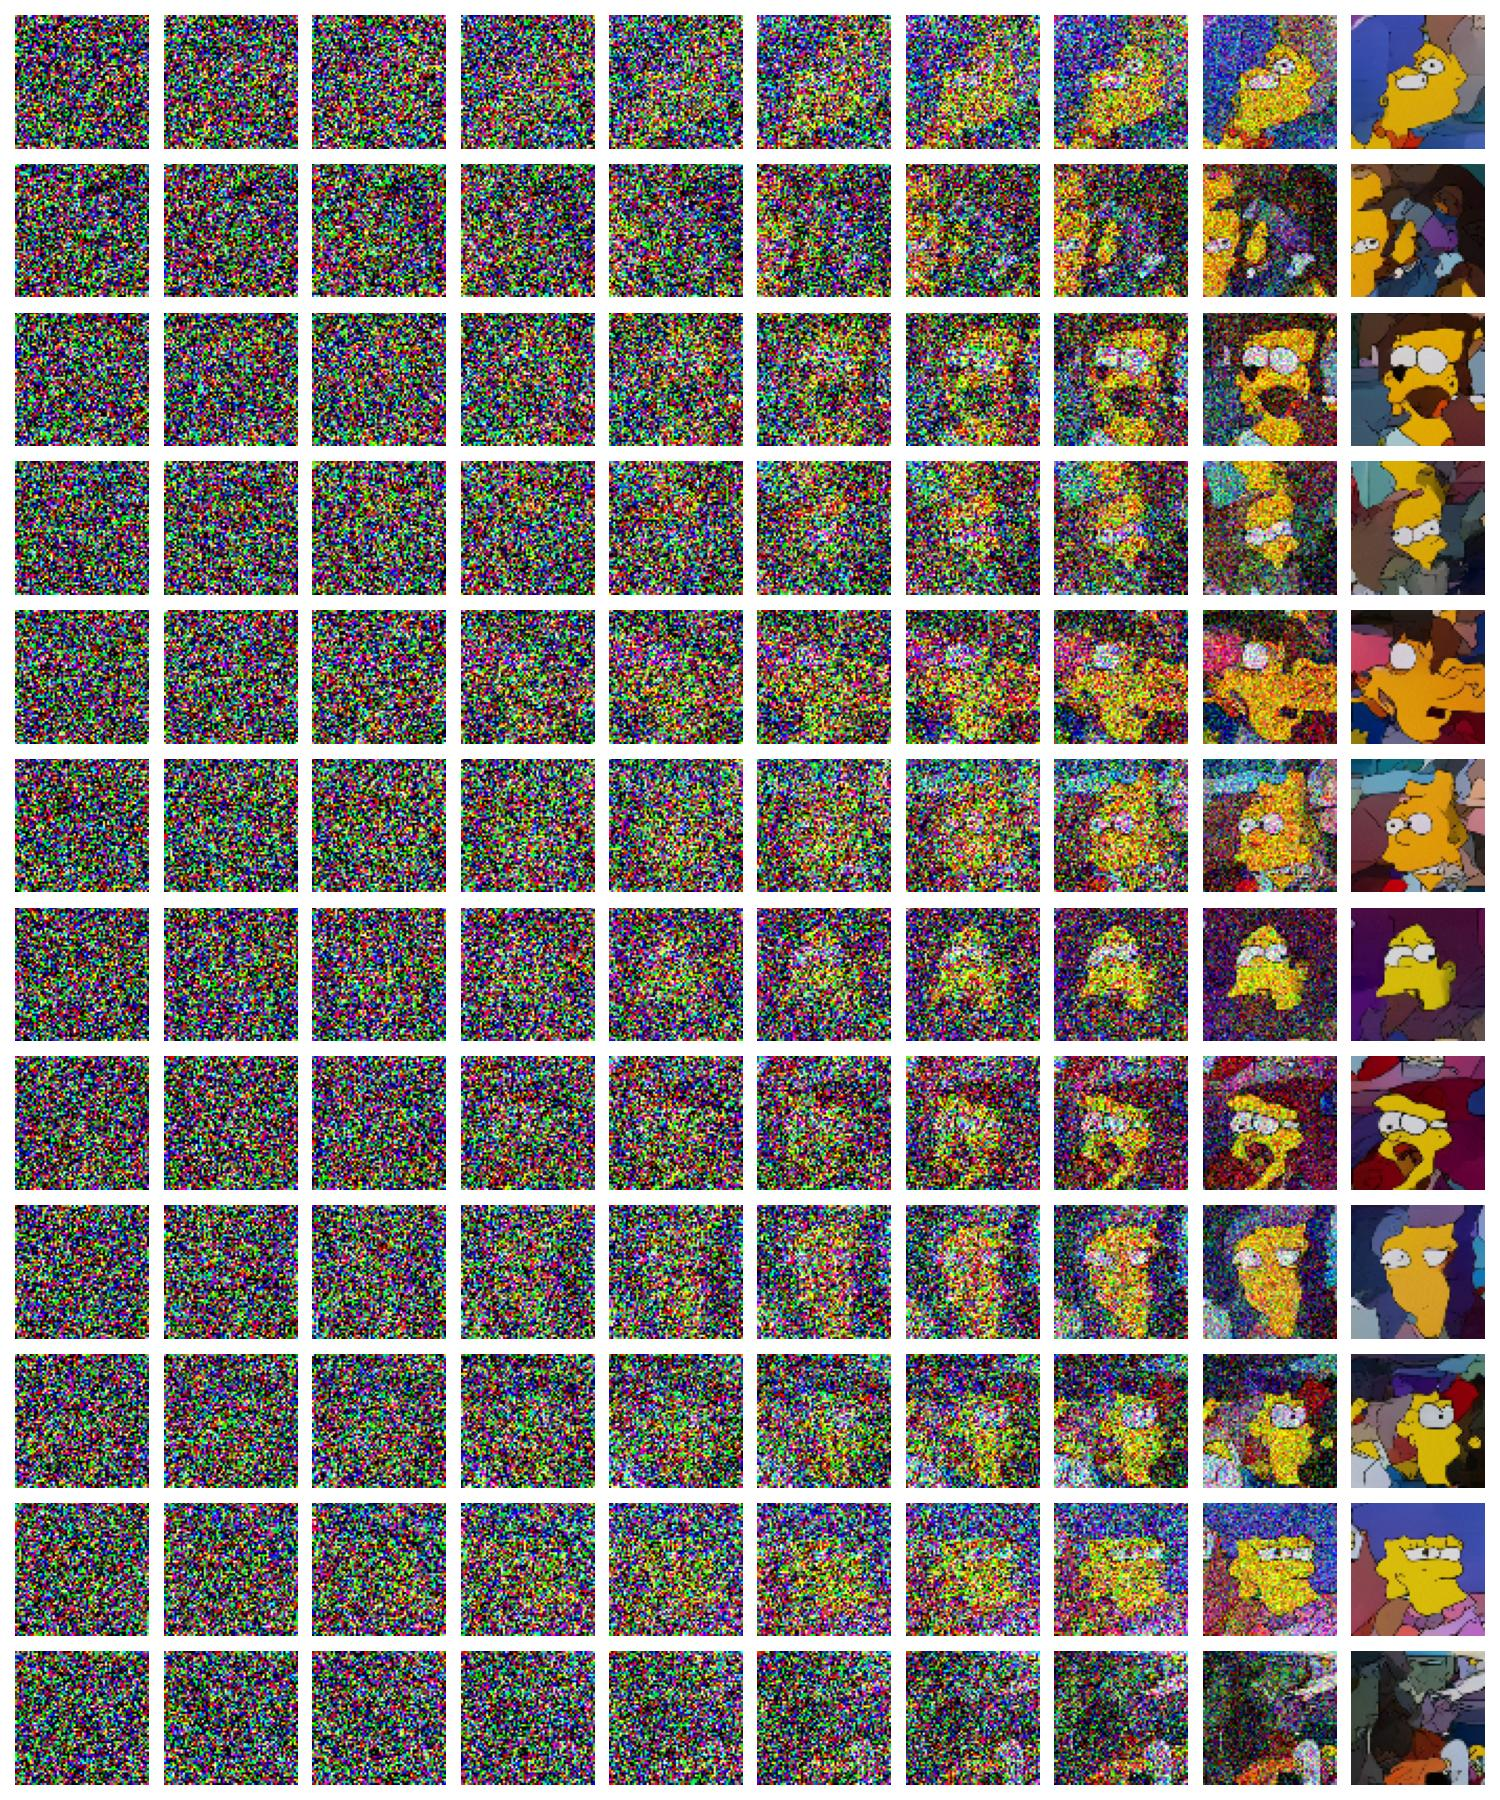
\includegraphics[width=1\textwidth]{simp64rev.jpg}
  \caption{drunkSimpson64 model reverse process, 75 step transitions, $t=750$, base\_channels = $512$, time\_emb\_dim = $512$, batch\_size = 16, lr$=1e^{-4}$, linear $\beta \in(1e^{-4}, 0.02)$}
\end{figure}

\begin{figure}[H]
  \centering
  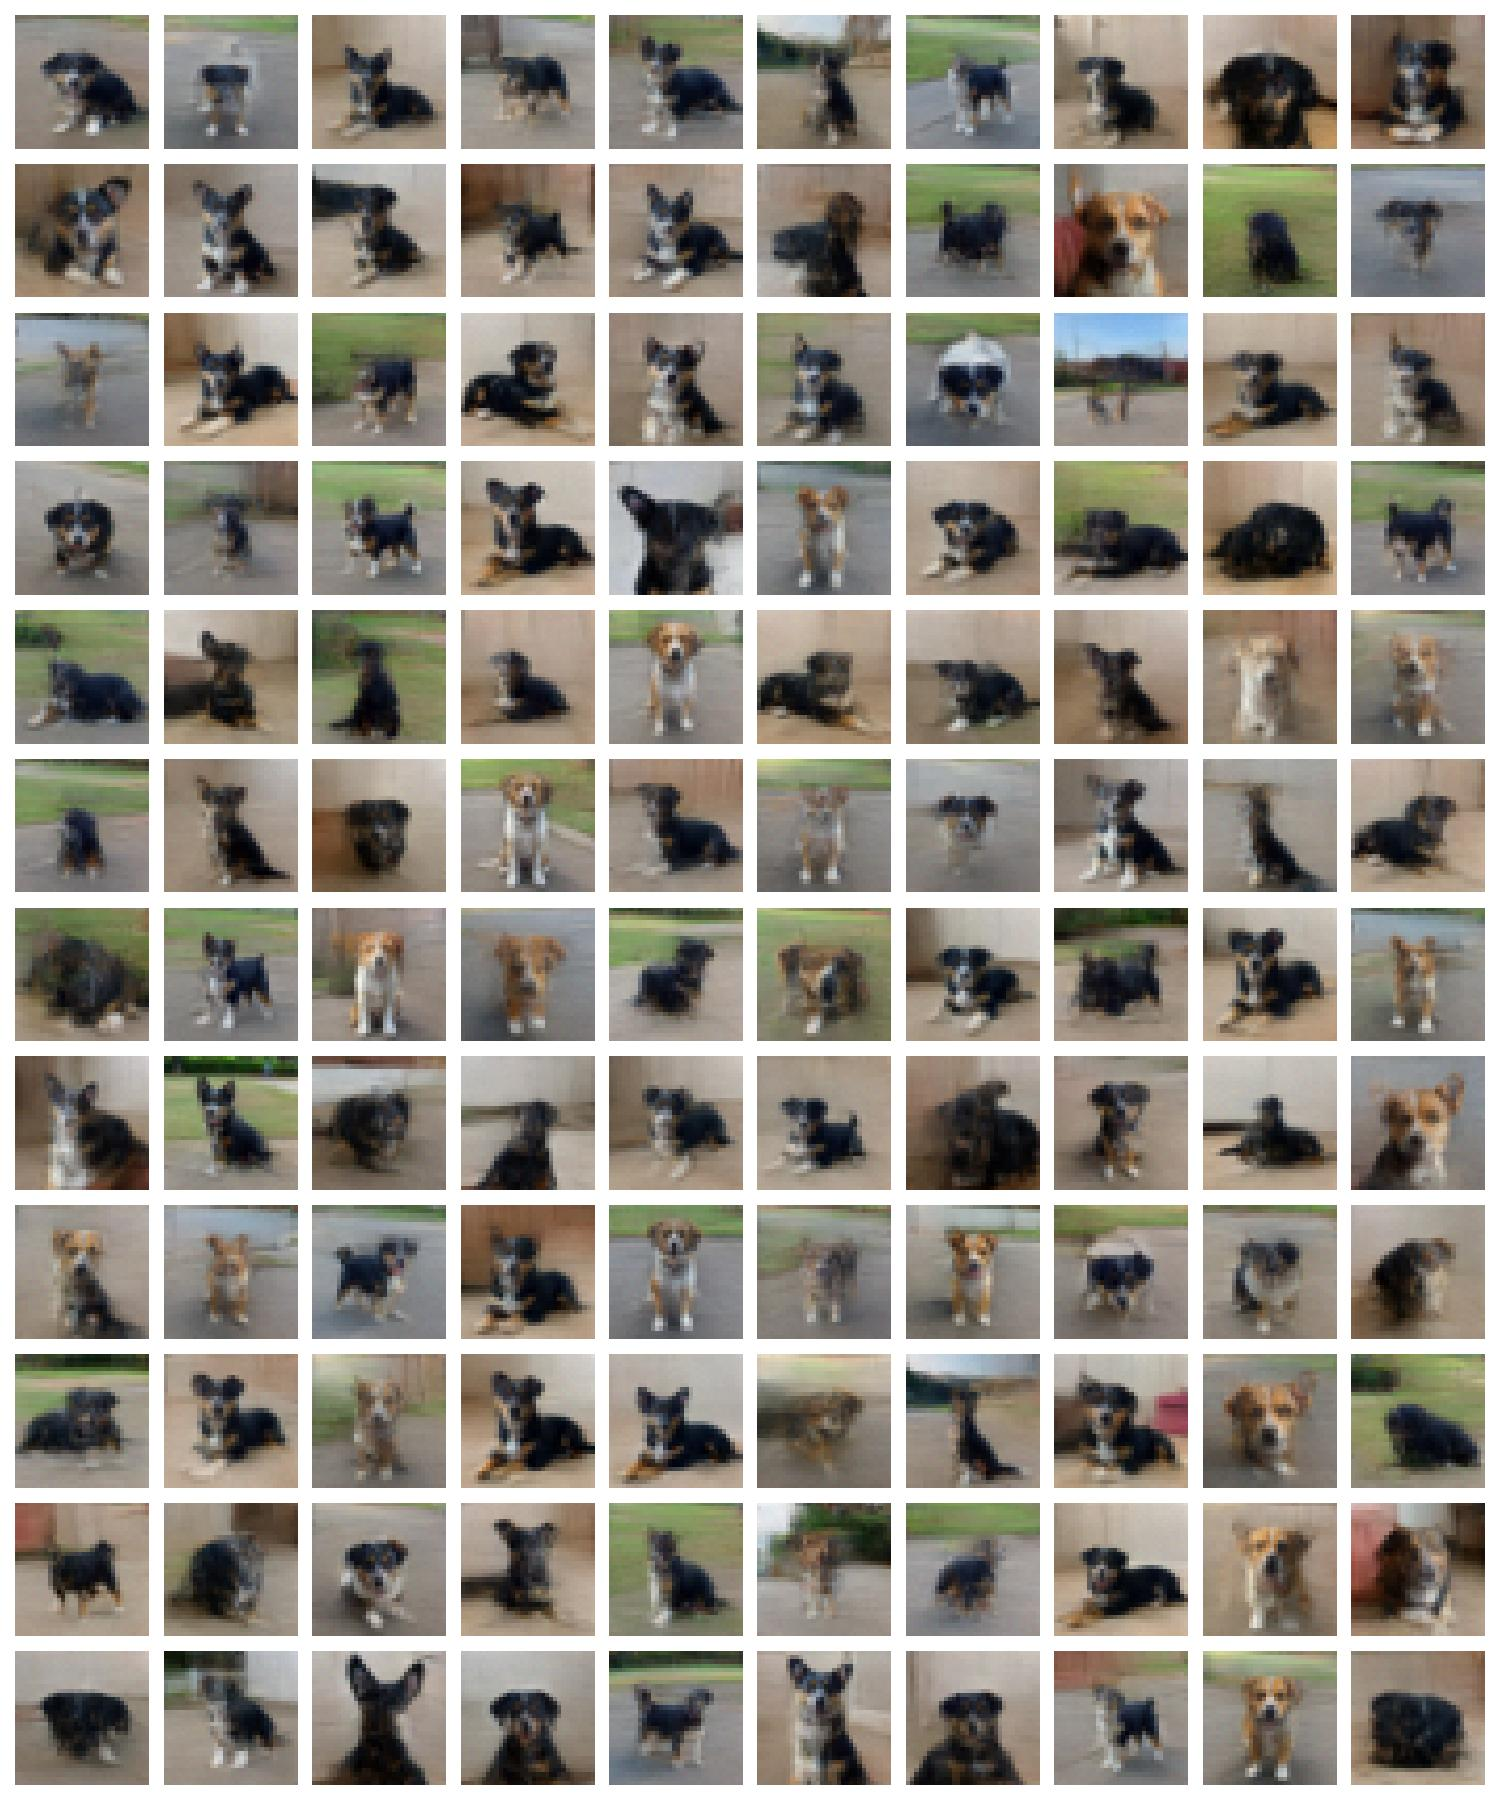
\includegraphics[width=1\textwidth]{dog32ext.jpg}
  \caption{dog32 model, $t=500$, base\_channels = $256$, time\_emb\_dim = $512$, batch\_size = 32, lr$=1e^{-4}$, linear $\beta \in(1e^{-4}, 0.02)$}
\end{figure}

\begin{figure}[H]
  \centering
  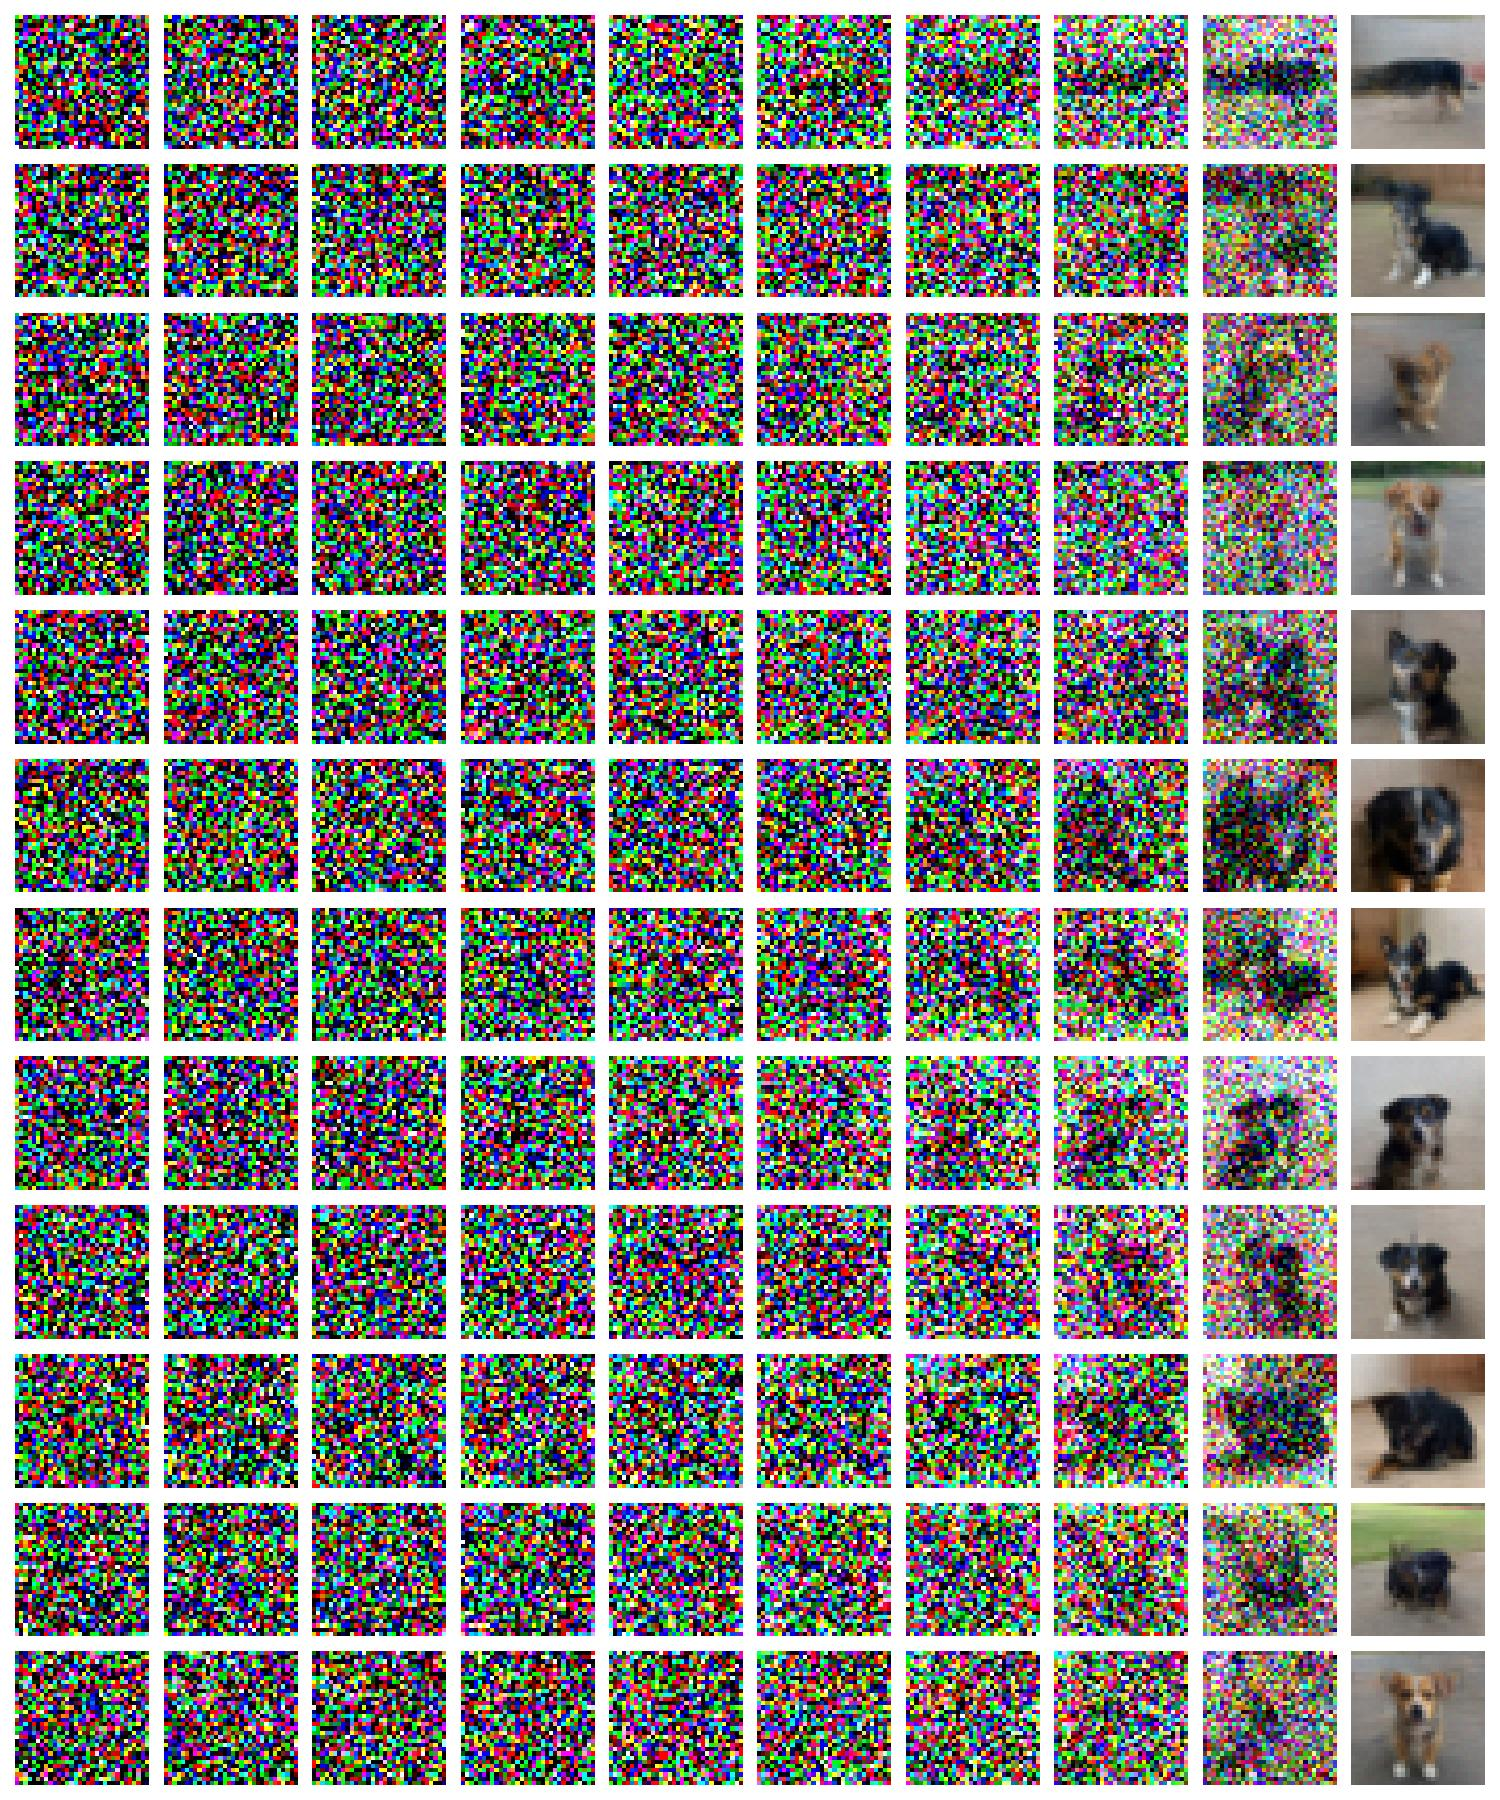
\includegraphics[width=1\textwidth]{dog32rev.jpg}
  \caption{dog32 model reverse process, 100 step transitions, $t=1000$, base\_channels = $256$, time\_emb\_dim = $512$, batch\_size = 32, lr$=1e^{-4}$, linear $\beta \in(1e^{-4}, 0.02)$}
\end{figure}

\end{document}
